% \documentclass{article}

% \documentclass{book}

\documentclass{report} % Chọn cỡ chữ

\usepackage{contents/start/init}

\usepackage{contents/start/vvn}

%%%%%%%%%%%%%%%%%%%%%%%%%%%%%%%%%%

\pagecolor[RGB]{40, 42, 54}% Đặt màu nền

\color[RGB]{18, 161, 24} % Đặt màu chữ

%%%%%%%%%%%%%%%%%%%%%%%%%%%%%%%%%%
\begin{document} % Bắt đầu

%%%%%%%%%%%%%%%%%%%%%%%%%%%%%%%%%%

% \begin{titlepage}

\begin{tikzpicture}[remember picture, overlay]\draw [line width = 3pt]($ (current page.north west) + (3.0cm, - 2.5cm)$)rectangle($ (current page.south east) + (- 2.5cm, 2.5cm)$);\draw [line width = 0.5pt]($ (current page.north west) + (3.1cm, - 2.6cm)$)rectangle($ (current page.south east) + (- 2.6cm, 2.6cm)$);\end{tikzpicture}

\begin{center}

\vspace{- 0.4cm}

\textbf{ĐẠI HỌC BÁCH KHOA HÀ NỘI} \\

\textbf{VIỆN TOÁN ỨNG DỤNG VÀ TIN HỌC} \\

\textbf{******}

\vspace{0.8cm}

\begin{figure}[H]

\centering


\includegraphics[scale = 0.5]{pictures/hust/main.png}

\end{figure}

\vspace{0.7cm}

\textbf{\fontsize{16pt}{30pt}\selectfont {BÁO CÁO ĐỒ ÁN II}} \\

\textbf{\fontsize{10pt}{24pt}\selectfont {CHUYÊN NGÀNH: TOÁN TIN}}

\vspace{1cm}

\textbf{\fontsize{16pt}{30pt}\selectfont {ĐỀ TÀI:}} \\

% \textbf{\fontsize{19pt}{24pt}\selectfont {Xây dựng kiến trúc vi dịch vụ cho \\ bài toán hóa đơn điện tử}} \\

\textbf{\fontsize{20pt}{24pt}\selectfont {Sử dụng thiết kế hướng miền \\ xây dựng kiến trúc vi dịch vụ cho \\ bài toán hóa đơn điện tử}} \\

\end{center}

\vspace{0.7cm}

\hspace{2.6cm}\begin{minipage}{0.8\textwidth}

\textbf{\fontsize{10pt}{24pt}\selectfont {Giảng viên hướng dẫn: TS. Vũ Thành Nam}}

\end{minipage}

\vspace{0.7cm}

\hspace{3cm}\begin{minipage}{0.7\textwidth}

\begin{tabular}{l l l}

\textbf{\fontsize{10pt}{24pt}\selectfont {Sinh viên thực hiện}} & \textbf{\fontsize{10pt}{24pt}\selectfont {Vũ Văn Nghĩa}} \\

\textbf{\fontsize{10pt}{24pt}\selectfont {Mã số sinh viên}} & \textbf{\fontsize{10pt}{24pt}\selectfont {20206205}} \\

\textbf{\fontsize{10pt}{24pt}\selectfont {Lớp}} & \textbf{\fontsize{10pt}{24pt}\selectfont {Toán Tin 02 - K65}} \\

\end{tabular}

\end{minipage}

\vspace{0.5cm}

\begin{center}

\textbf{Hà Nội, \the\month~/~\the\year}

\end{center}

\end{titlepage}



% % % Trang trắng không có nội dung và không có số trang

% \pagestyle{empty}

% \thispagestyle{empty}

% \mbox{} % Một hộp rỗng để trang không bị trắng toàn bộ


 



%%%%%%%%%%%%%%%%%%%%%%%%%%%%%%%%%%


% \newpage


% Trang trắng
\blankpage


% \begin{titlepage}

\begin{tikzpicture}[remember picture, overlay]\draw [line width = 3pt]($ (current page.north west) + (3.0cm, - 2.5cm)$)rectangle($ (current page.south east) + (- 2.5cm, 2.5cm)$);\draw [line width = 0.5pt]($ (current page.north west) + (3.1cm, - 2.6cm)$)rectangle($ (current page.south east) + (- 2.6cm, 2.6cm)$);\end{tikzpicture}

\begin{center}

\vspace{- 0.4cm}

\textbf{ĐẠI HỌC BÁCH KHOA HÀ NỘI} \\

\textbf{VIỆN TOÁN ỨNG DỤNG VÀ TIN HỌC} \\

\textbf{******}

\vspace{0.8cm}

\begin{figure}[H]

\centering


\includegraphics[scale = 0.5]{pictures/hust/main.png}

\end{figure}

\vspace{0.7cm}

\textbf{\fontsize{16pt}{30pt}\selectfont {BÁO CÁO ĐỒ ÁN II}} \\

\textbf{\fontsize{10pt}{24pt}\selectfont {CHUYÊN NGÀNH: TOÁN TIN}}

\vspace{1cm}

\textbf{\fontsize{16pt}{30pt}\selectfont {ĐỀ TÀI:}} \\

% \textbf{\fontsize{19pt}{24pt}\selectfont {Xây dựng kiến trúc vi dịch vụ cho \\ bài toán hóa đơn điện tử}} \\

\textbf{\fontsize{20pt}{24pt}\selectfont {Sử dụng thiết kế hướng miền \\ xây dựng kiến trúc vi dịch vụ cho \\ bài toán hóa đơn điện tử}} \\

\end{center}

\vspace{0.7cm}

\hspace{2.6cm}\begin{minipage}{0.8\textwidth}

\textbf{\fontsize{10pt}{24pt}\selectfont {Giảng viên hướng dẫn: TS. Vũ Thành Nam}}

\end{minipage}

\vspace{0.7cm}

\hspace{3cm}\begin{minipage}{0.7\textwidth}

\begin{tabular}{l l l}

\textbf{\fontsize{10pt}{24pt}\selectfont {Sinh viên thực hiện}} & \textbf{\fontsize{10pt}{24pt}\selectfont {Vũ Văn Nghĩa}} \\

\textbf{\fontsize{10pt}{24pt}\selectfont {Mã số sinh viên}} & \textbf{\fontsize{10pt}{24pt}\selectfont {20206205}} \\

\textbf{\fontsize{10pt}{24pt}\selectfont {Lớp}} & \textbf{\fontsize{10pt}{24pt}\selectfont {Toán Tin 02 - K65}} \\

\end{tabular}

\end{minipage}

\vspace{0.5cm}

\begin{center}

\textbf{Hà Nội, \the\month~/~\the\year}

\end{center}

\end{titlepage}



% % % Trang trắng không có nội dung và không có số trang

% \pagestyle{empty}

% \thispagestyle{empty}

% \mbox{} % Một hộp rỗng để trang không bị trắng toàn bộ


 



%%%%%%%%%%%%%%%%%%%%%%%%%%%%%%%%%%


% \newpage


% Trang trắng
\blankpage


% % \newpage

\begin{center}

    {\bfseries NHẬN XÉT CỦA GIẢNG VIÊN HƯỚNG DẪN}
    
    \end{center}
    
    \begin{enumerate}
    
    \item Mục đích và nội dung của đồ án:
    
    \vspace{20ex} % Thêm khoảng cách dọc
    
    \item 	Kết quả đạt được:
    
    \vspace{20ex} % Thêm khoảng cách dọc
    
    \item 	Ý thức làm việc của sinh viên:
    
    \vspace{20ex} % Thêm khoảng cách dọc
    
    \end{enumerate}
    
    \hspace{0.4\textwidth}\begin{minipage}{0.5\textwidth}
    
    \noindent\begin{center}
    
    \textit{Hà Nội, \today} \\
    
    \textbf{Giảng viên hướng dẫn} \\
    
    \textit{(Ký và ghi rõ họ tên)}
    
    \vspace{2cm}
    
    \textbf{TS. Vũ Thành Nam}
    
    \end{center}
    
    \end{minipage}
    
    \pagestyle{empty}
    
    % \newpage
    
    

% 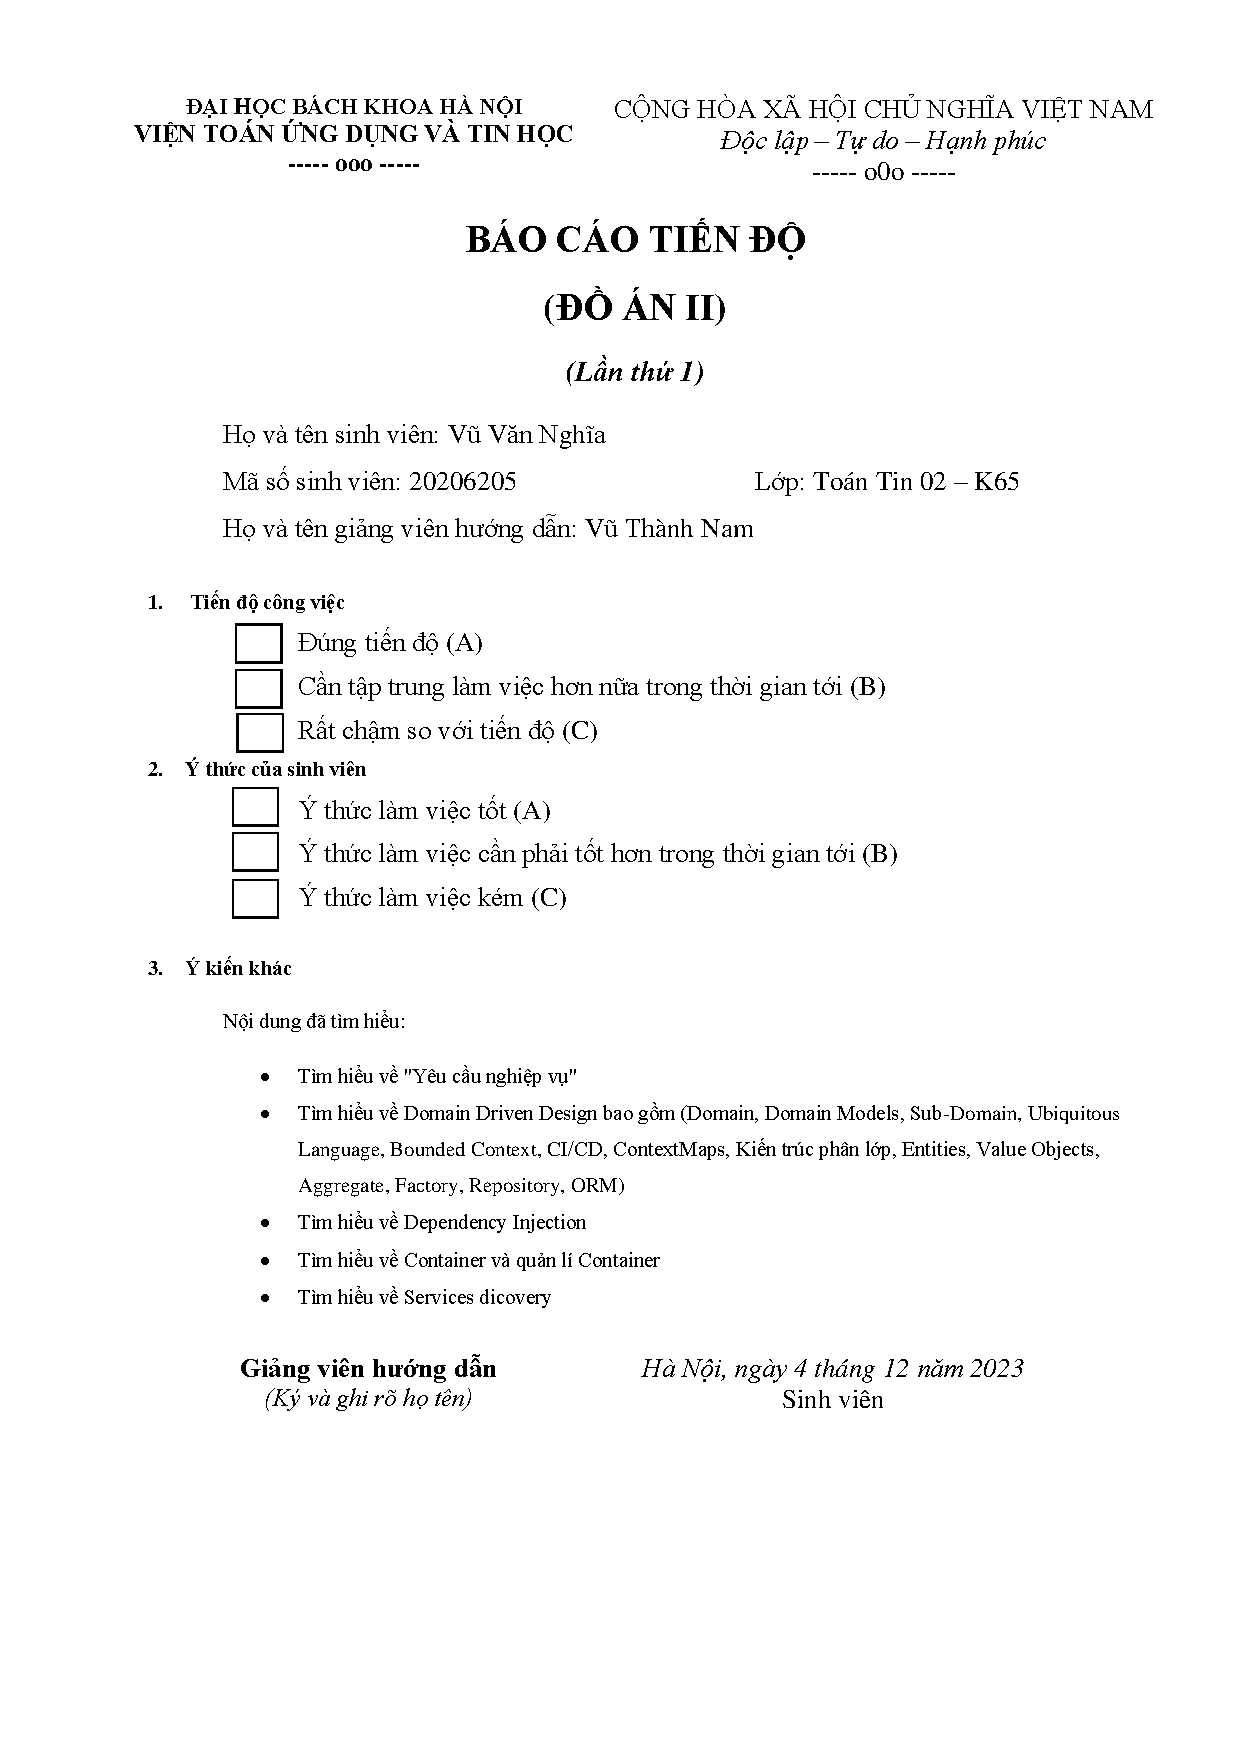
\includepdf[pages = -]{contents/bao_cao_tien_do_1.pdf}

% 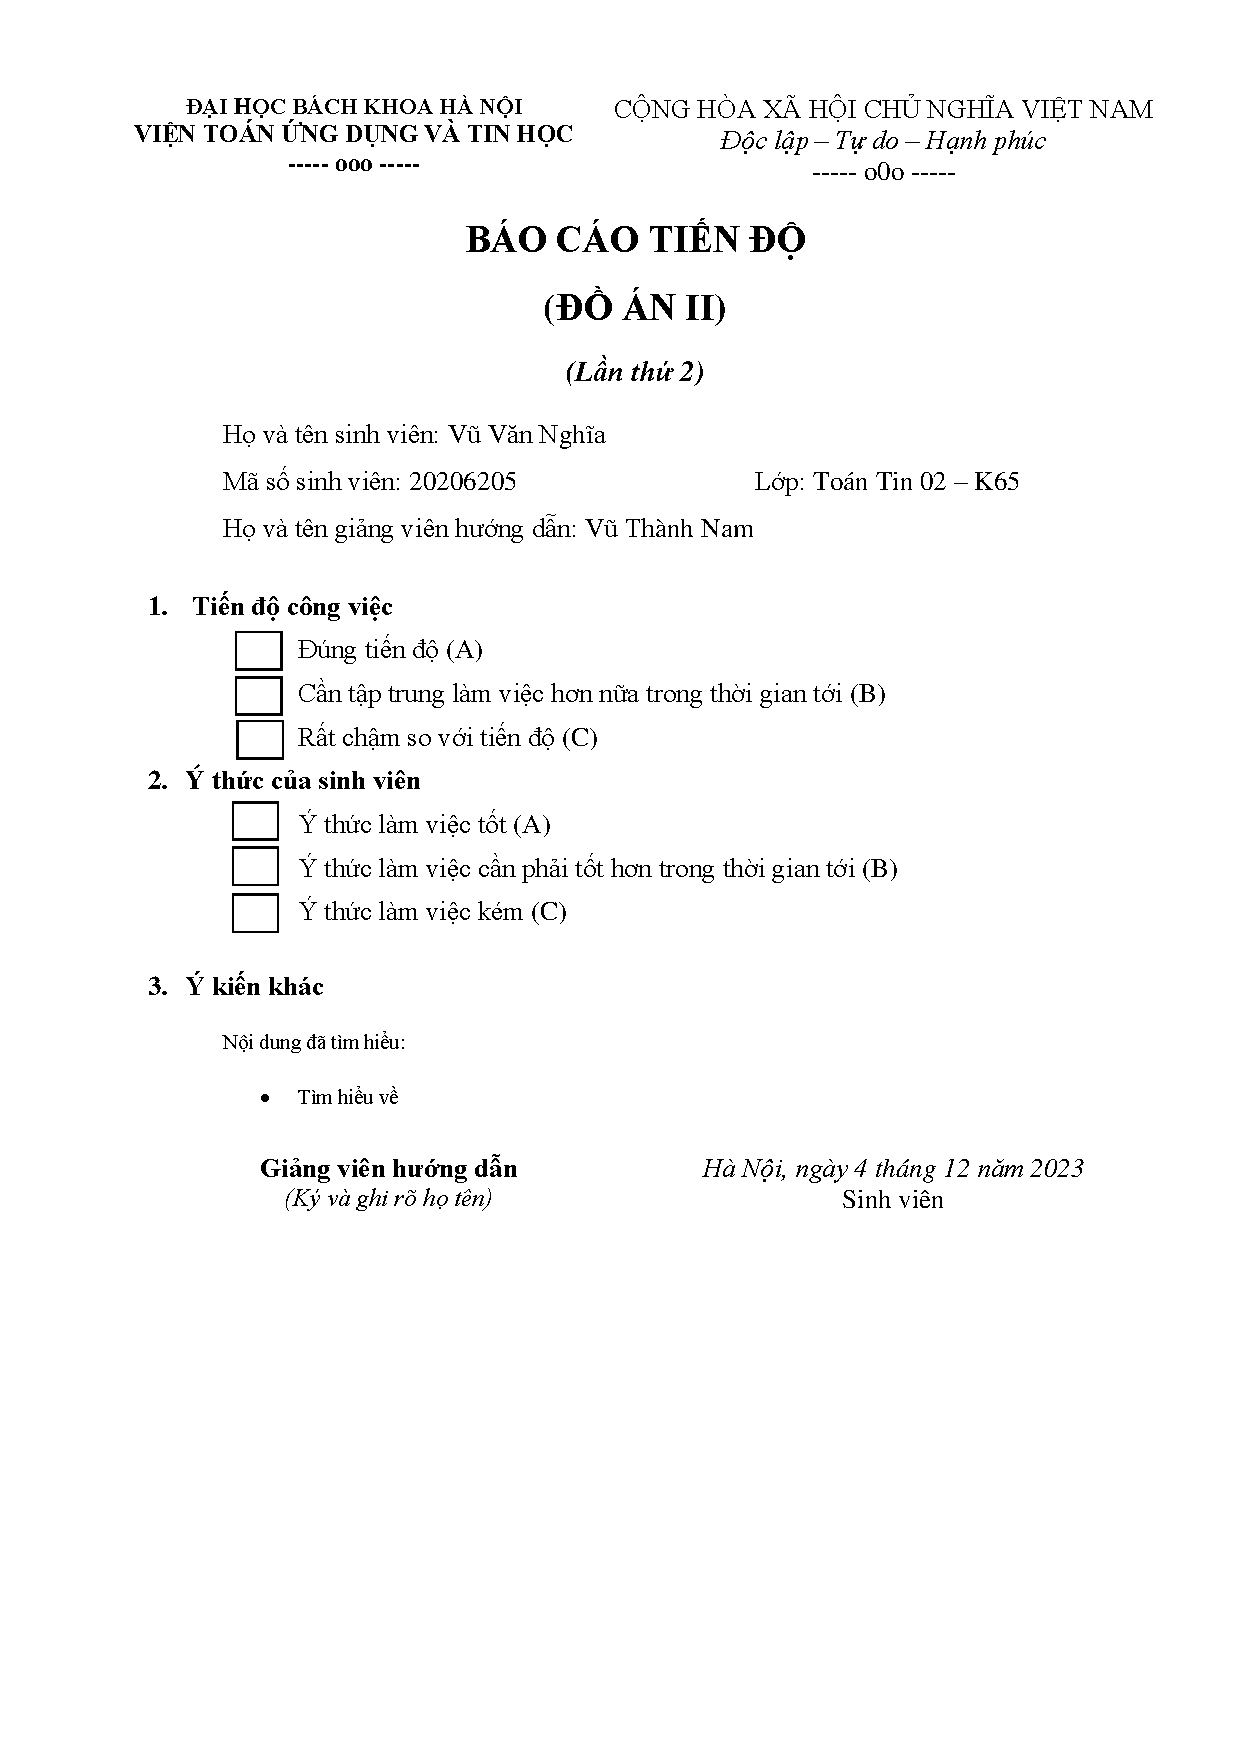
\includepdf[pages = -]{contents/bao_cao_tien_do_2.pdf}

%%%%%%%%%%%%%%%%%%%%%%%%%%%%%%%%%%

% 
\renewcommand*\contentsname{\centering MỤC LỤC}

\tableofcontents

\setcounter{page}{0}




%%%%%%%%%%%%%%%%%%%%%%%%%%%%%%%%%%

% \newpage

\section*{\centering LỜI CẢM ƠN}

\addcontentsline{toc}{section}{LỜI CẢM ƠN}

\blindtext % Tạo văn bản ngẫu nhiên

\newpage



% \newpage

\section*{\centering DANH SÁCH BẢNG}

\addcontentsline{toc}{section}{DANH SÁCH BẢNG}

\makeatletter

\renewcommand\listoftables{

\@starttoc{lot}

}

\makeatother

\listoftables

\newpage

% \chapter*{\centering DANH SÁCH HÌNH ẢNH}

\addcontentsline{toc}{chapter}{DANH SÁCH HÌNH ẢNH}

\makeatletter

\renewcommand\listoffigures{

\@starttoc{lof}

}

\makeatother

\listoffigures



% \newpage

\section*{\centering DANH SÁCH CÁC CỤM TỪ VIẾT TẮT}

\addcontentsline{toc}{section}{DANH SÁCH CÁC CỤM TỪ VIẾT TẮT}

% @sau

\begin{table}[h]

\centering

\begin{tabular}{|c|c|c|c|}

\hline

STT & Từ viết tắt & Từ viết đầy đủ & Mô tả \\

\hline

Dong1 & Dong1 & Cot1 & Cot2 \\

\hline

Dong2 & Dong2 & Cot1 & Cot2 \\

\hline

\end{tabular}

\end{table}

\newpage

% API; Application Programming Interface; Giao diện lập trình ứng dụng

% CI/CD; Continuous Integration (CI) and Continuous Delivery (CD) ; Quá trình tích hợp và chuyển giao liên tục

% thiết kế hướng miền ; thiết kế hướng miền; Kỹ thuật thiết kế theo hướng miền

% DI; Dependency Injection; Cơ chế tiêm sự phụ thuộc giữa các đối tượng

% HTTP; Hypertext Transfer Protocol; Giao thức truyền tải siêu văn bản

% JSON; JavaScript Object Notation; Một kiểu dữ liệu mở rộng của JavaScript

% ORM; Object Relational Mapping; Một kỹ thuật ánh xạ các đối tượng lập trình với từng bảng trong CSDL quan hệ

% Cơ sở dữ liệu ; CSDL ;

% Tạo (Create), Đọc (Read), Sửa (Update), Xóa (Delete) ; CRUD ;

% Kubernetes ; K8s ; kubernetes

% Số điện thoại ; SĐT ;

% UML

% MVC; Model View Controller; Một mẫu thiết kế ứng dụng

% SQL

SOA; Service Oriented Architecture; Kiến trúc hướng dịch vụ

SOAP; Simple Object Access Protocol; Một giao thức để truy cập dịch vụ web

SPA; Single Page Application; Kiểu ứng dụng một trang

REST; Representational State Transfer; Một tiêu chuẩn thiết kế các API sử dụng cho các dịch vụ web

URL; Uniform Resource Locator ; Địa chỉ định vị tài nguyên trên Internet

XML; Extensible Markup Language; Ngôn ngữ đánh dấu mở rộng

% TCT ; TCT ;

Người nộp thuế ; NNT ;

Mã số thuế ; MST ;

Hóa đơn điện tử ; HĐĐT ;

Cơ quan thuế ; CQT ;

Công nghệ thông tin ; CNTT ;



% \newpage

\section*{\centering DANH SÁCH CÁC THUẬT NGỮ}

\addcontentsline{toc}{section}{DANH SÁCH CÁC THUẬT NGỮ}

% @sau

% @sau

\begin{table}[h]

\centering

\begin{tabular}{|c|c|c|}

\hline

STT & Tiếng Anh & Tiếng Việt \\

\hline

Dong1 & Dong1 & Cot2 \\

\hline

Dong2 & Dong2 & Cot2 \\

\hline

\end{tabular}

\end{table}

\newpage

% kiến trúc nguyên khối, kiến trúc nguyên khối

% kiến trúc nguyên khối, kiến trúc nguyên khối

% kiến trúc vi dịch, kiến trúc vi dịch

% kiến trúc vi dịch, kiến trúc vi dịch

% kiến trúc vi dịch, kiến trúc vi dịch

% kiến trúc vi dịch, kiến trúc vi dịch

% thiết kế hướng miền, thiết kế hướng miền

% thiết kế hướng miền, thiết kế hướng miền

1 thiết kế hướng miền

Thiết kế hướng lĩnh vực

2 Domain (không dịch)

3 Abstraction Trừu tượng

4 chuyên gia ngành

%%%%%%%%%%%%%%%%%%%%%%%%%%%%%%%%%%

% \chapter*{\centering MỞ ĐẦU}

% \addcontentsline{toc}{chapter}{MỞ ĐẦU}

% \section*{Lý do chọn đề tài}

% Trong quá trình hoạt động kinh doanh, doanh nghiệp có nhu cầu chuyển đổi mô hình kinh doanh linh hoạt để có thể tồn tại và phát triển khi thị trường thay đổi. Từ đó, đáp ứng nhu cầu của khách hàng, mang lại ưu thế cạnh tranh so với các đối thủ.

Trong những năm gần đây, việc áp dụng kiến trúc vi dịch vụ ngày càng phổ biến, đem lại nhiều lợi ích như tách các nghiệp vụ kinh doanh thành các dịch vụ nhỏ độc lập, tăng tính linh hoạt và khả năng chống chịu sự cố.

Kiến trúc vi dịch vụ hỗ trợ doanh nghiệp chuyển đổi nhanh chóng để đáp ứng nhu cầu của mô hình kinh doanh và mong đợi của khách hàng. Tuy nhiên, để xây dựng được kiến trúc vi dịch vụ tốt, cần phải tạo ra các dịch vụ nhỏ phù hợp và duy trì tính độc lập. Trong đồ án này, em sử dụng thiết kế hướng miền để phân tích và xây dựng kiến trúc vi dịch vụ.

Theo quy định của Nghị định 123/2020/NĐ - CP, tất cả các doanh nghiệp, tổ chức và hộ kinh doanh đều bắt buộc phải sử dụng hóa điện tử. Vì vậy, nhu cầu sử dụng và xử lý hóa đơn điện tử trở nên rất lớn. Do đó trong đồ án này, em chọn chủ đề \emph{"Sử dụng thiết kế hướng miền xây dựng kiến trúc vi dịch vụ cho bài toán hóa đơn điện tử"}. Chủ đề này là một xu hướng quan trọng trong phát triển phần mềm và mang lại nhiều lợi ích trong việc cải thiện quá trình quản lý hóa đơn điện tử.



% \section*{Đối tượng và phạm vi nghiên cứu}

% \begin{itemize}

\item \textbf{Đối tượng nghiên cứu:} Kiến trúc vi dịch vụ

\item \textbf{Phạm vi nghiên cứu:} Tập trung vào tìm hiểu thiết kế hướng miền xây dựng kiến trúc vi dịch vụ cho bài toán hóa đơn điện tử.

\end{itemize}



% \section*{Tóm tắt nội dung đồ án}

% Báo cáo đồ án này được tổ chức thành các phần chính sau:

\begin{itemize}

\item \textbf{Chương 1: Phân tích thiết kế hệ thống}

\begin{quote}

Nội dung phân tích hệ thống bán hàng.

\end{quote}

\item \textbf{Chương 2: Trình bày về kiến trúc kiến trúc vi dịch vụ}

\begin{quote}

Trình bày các công nghệ, kĩ thuật, nội dung của kiến trúc kiến trúc vi dịch vụ.

\end{quote}

\item \textbf{Chương 3: Các công nghệ đã sử dụng}

\begin{quote}

Trình bày các công nghệ em đã sử dụng trong đồ án này.

\end{quote}

\end{itemize}

%@ Thêm các mục nhỏ như:
%@ Thêm các mục nhỏ như:
%@ Thêm các mục nhỏ như:
%@ Thêm các mục nhỏ như:
%@ Thêm các mục nhỏ như:
%@ Thêm các mục nhỏ như:
%@ Thêm các mục nhỏ như:
%@ Thêm các mục nhỏ như:
%@ Thêm các mục nhỏ như:
%@ Thêm các mục nhỏ như:
%@ Thêm các mục nhỏ như:
%@ Thêm các mục nhỏ như:
%@ Thêm các mục nhỏ như:

% Luận văn được tổ chức thành các phần chính sau:

% Mở đầu: Trình bày tổng quan về đề tài

% Chương 1: Trình bày cách thức phát triển phần mềm theo kiến trúc kiến trúc vi dịch vụ .

% Trong chương này, luận văn tập trung làm rõ các nội dung:

% - Sơ lược về một số hướng kiến trúc phần mềm truyền thống như kiến trúc nguyên

% khối, kiến trúc hướng dịch vụ, công nghệ ESB

% - Tổng quan về kiến trúc kiến trúc vi dịch vụ : sự ra đời, đặc điểm của kiến trúc vi dịch vụ

% - Các mẫu thiết kế quan trọng được sử dụng trong kiến trúc vi dịch vụ

% - Một số nguyên tắc thiết kế kiến trúc vi dịch vụ

% Chương 2: Trình bày hướng xây dựng ứng dụng web sử dụng micro - frontends.

% Trong chương này, luận văn tập trung làm rõ các nội dung:

% - Sơ lược về một số mô hình phát triển web như mô hình web tĩnh, mô hình web

% động, mô hình web theo hướng SPA

% - Sự ra đời của kiến trúc micro - frontends

% - Các cơ chế tích hợp micro - frontends được thảo luận như: tích hợp theo hướng

% “build - time”, tích hợp theo hướng “run - time”, cách thức điều hướng và giao tiếp

% giữa các micro - frontends

% Chương 3: Trình bày cách thức xây dựng một ứng dụng thử nghiệm sử dụng kiến

% trúc kiến trúc vi dịch vụ, micro - frontends. Một số nội dung chính trong quá trình thực nghiệm

% được làm rõ bao gồm:

% 3

% - Áp dụng phương pháp thiết kế hướng miền để phân hoạch, thiết kế chương trình

% - Thiết kế và cài đặt tầng dịch vụ theo hướng kiến trúc vi dịch vụ, sử dụng các công

% nghệ trên nền tảng Java như Spring Boot, Spring Cloud

% - Thiết kế và cài đặt tầng giao diện theo hướng micro - frontends, sử dụng các công

% nghệ như Single - SPA, Angular, ReactJS

% - Một số kỹ thuật kiểm thử kiến trúc vi dịch vụ cũng được thảo luận như kiểm thử đơn

% vị, kiểm thử tích hợp và kiểm thử mức giao diện

% - Cách thức triển khai ứng dụng sử dụng Docker

% Phần kết luận: Tổng kết, đánh giá kết quả thu được của quá trình nghiên cứu cũng

% như các ưu nhược điểm, các hạn chế và hướng phát triển tương lai.

% @ Trong quá trình hoàn thành bài báo cáo này không tránh khỏi những thiếu sót. Vì vậy, em mong nhận được sự giúp đỡ và ý kiến đóng góp chân thành từ các thầy cô để em có thể cải thiện và hoàn thiện đề tài này một cách tốt nhất. Sự đóng góp quý báu của các thầy cô sẽ giúp em hiểu sâu hơn về đề tài và nắm vững hơn trong quá trình thực hiện.

%%%%%%%%%%%%%%%%%%%%%%%%%%%%%%%%%%

% \chapter{Giới thiệu chung}

% Trong thời đại ngày nay, nhu cầu phát triển ứng dụng và hệ thống ngày càng tăng, đặt ra thách thức đối với kiến trúc phần mềm. Kiến trúc nguyên khối đã phục vụ hiệu quả trong quá khứ, nhưng kiến trúc này bắt đầu gặp khó khăn khi đối mặt với sự phức tạp, khả năng mở rộng và khả năng đáp ứng linh hoạt với sự thay đổi nhanh chóng trong yêu cầu kinh doanh.

Kiến trúc vi dịch vụ là giải pháp cho những thách thức trên. Kiến trúc vi dịch vụ chia dự án thành những dịch vụ nhỏ độc lập, mỗi dịch vụ chịu trách nhiệm về một chức năng cụ thể. Từ đó, dự án giảm sự phức tạp, tăng tính linh hoạt và dễ dàng quản lý.

Việc vận dụng kết hợp giữa kiến trúc vi dịch vụ và thiết kế hướng miền là một cách tiếp cận toàn diện, giúp xác định và tổ chức các dịch vụ dựa trên việc hiểu rõ về lĩnh vực kinh doanh. Thiết kế hướng miền xây dựng mô hình dựa trên yêu cầu nghiệp vụ thực tế, từ đó dự án phản ánh đúng các quy trình kinh doanh.



Trong quá trình hoạt động kinh doanh, không phải mọi doanh nghiệp đều giữ nguyên mô hình kinh doanh được đưa ra ban đầu của mình. Khi quy mô thị trường thay đổi, việc chuyển đổi mô hình kinh doanh là điều cần thiết. Chuyển đổi kinh doanh như một công cụ linh hoạt giúp các doanh nghiệp có thể phát triển và tồn tại giữa các đối thủ của mình.

\begin{example}

\begin{itemize}

\item Google bắt đầu như công cụ tìm kiếm trực tuyến, nhưng sau đó đã mở rộng và thay đổi mô hình kinh doanh qua nhiều dịch vụ và sản phẩm khác nhau như: Dịch vụ đám mây Google Cloud Platform, Dịch vụ thư điện tử Gmail, Dịch vụ bản đồ Google Maps, Dịch vụ lưu trữ tập tin Google Drive, \dots

\item Amazon từ hiệu sách trực tuyến đã trở thành thị trường cho nhà cung cấp khác như: Thương mại điện tử, Dịch vụ đám mây Amazon Web Services (AWS), \dots

\begin{figure}[H]

\centering


\includegraphics[scale = 0.5]{pictures/kien_truc_vi_dich_vu_cua_amazon/main.png}

\caption{Kiến trúc vi dịch vụ của Amazon}

\end{figure}

\end{itemize}

\end{example}

Đối với những doanh nghiệp không chuyển đổi kinh doanh sẽ không thể tồn tại.

\begin{example} Gần đây, dịch vụ giao đồ ăn Baemin đã rời khỏi thị trường Việt Nam cũng do sức ép từ các đối thủ khác khiến Baemin khó cạnh tranh trong mảng kinh doanh cốt lõi là giao đồ ăn. Các đối thủ này không chỉ cung cấp dịch vụ giao đồ ăn mà còn có đặt xe, giao hàng,...

\end{example}

\begin{figure}[H]

\centering


\includegraphics[scale = 0.5]{pictures/baemin/main.png}

\caption{Dịch vụ giao đồ ăn Baemin đã rời khỏi thị trường Việt Nam}

\end{figure}

Hiện nay, các tổ chức doanh nghiệp có nhu cầu chuyển đổi kinh doanh để có thể tồn tại và phát triển khi thị trường thay đổi. Từ đó, đáp ứng nhu cầu của khách hàng, mang lại ưu thế cạnh tranh so với các đối thủ. Do đó, các doanh nghiệp cần hệ thống chuyển đổi nhanh chóng để đáp ứng nhu cầu của mô hình kinh doanh và mong đợi của khách hàng.






Kiến trúc vi dịch vụ giải quyết những thách thức và hỗ trợ doanh nghiệp chuyển đổi kinh doanh, mở rộng hệ thống dễ dàng. Tuy nhiên, để xây dựng được một kiến trúc vi dịch vụ tốt, cần phải tạo ra các dịch vụ nhỏ phù hợp và duy trì tính độc lập. Trong đồ án này, em sử dụng thiết kế hướng miền để phân tích và xây dựng kiến trúc vi dịch vụ. Thiết kế hướng miền giúp xác định và tổ chức các dịch vụ dựa trên việc hiểu rõ về lĩnh vực kinh doanh, từ đó giúp dự án phản ánh chính xác các quy trình và quy tắc kinh doanh.



% \section{Giới thiệu về bài toán hóa đơn điện tử}

% Bài toán hóa đơn điện tử là một phần quan trọng của quá trình chuyển đổi số. Trong quá khứ, mọi người thường sử dụng hóa đơn giấy truyền thống. Ngày nay, khi có quy định kế toán và quản lý tài chính, hóa đơn điện tử đã trở nên phổ biến giúp giảm bớt sự phụ thuộc vào giấy tờ. Cùng với sự phát triển của khoa học công nghệ đã giúp quản lý hiệu quả công việc và tối ưu hóa quy trình kế toán và tài chính.



% \emph{Theo em tìm hiểu có các khái niệm và căn cứ pháp lý liên quan sau đây:}

% \subsection{Hóa đơn}

% \emph{Theo quy định tại khoản 1 Điều 3 Nghị định 123/2020/NĐ - CP:}

% %%%%%%%%%%%%%%%%%%%%%%%%%%%%%%%%%%%%%!

Hóa đơn là chứng từ kế toán do tổ chức, cá nhân bán hàng hóa, cung cấp dịch vụ lập, ghi nhận thông tin bán hàng hóa, cung cấp dịch vụ. Hóa đơn được thể hiện theo hình thức hóa đơn điện tử hoặc hóa đơn do cơ quan thuế đặt in.

%%%%%%%%%%%%%%%%%%%%%%%%%%%%%%%%%%%%%!



% \subsection{Hóa đơn điện tử}

% \emph{Theo quy định tại khoản 2 Điều 3 Nghị định 123/2020/NĐ - CP:}

% %%%%%%%%%%%%%%%%%%%%%%%%%%%%%%%%%%%%%!

Hóa đơn điện tử là hóa đơn có mã hoặc không có mã của cơ quan thuế được thể hiện ở dạng dữ liệu điện tử do tổ chức, cá nhân bán hàng hóa, cung cấp dịch vụ lập bằng phương tiện điện tử để ghi nhận thông tin bán hàng hóa, cung cấp dịch vụ theo quy định của pháp luật về kế toán, pháp luật về thuế, bao gồm cả trường hợp hóa đơn được khởi tạo từ máy tính tiền có kết nối chuyển dữ liệu điện tử với cơ quan thuế, trong đó:

a. Hóa đơn điện tử có mã của cơ quan thuế là hóa đơn điện tử được cơ quan thuế cấp mã trước khi tổ chức, cá nhân bán hàng hóa, cung cấp dịch vụ gửi cho người mua. Mã của cơ quan thuế trên hóa đơn điện tử bao gồm số giao dịch là một dãy số duy nhất do hệ thống của cơ quan thuế tạo ra và một chuỗi ký tự được cơ quan thuế mã hóa dựa trên thông tin của người bán lập trên hóa đơn.

b. Hóa đơn điện tử không có mã của cơ quan thuế là hóa đơn điện tử do tổ chức bán hàng hóa, cung cấp dịch vụ gửi cho người mua không có mã của cơ quan thuế.

%%%%%%%%%%%%%%%%%%%%%%%%%%%%%%%%%%%%%!



% \subsection{Bắt buộc sử dụng hóa đơn điện tử từ 01/07/2022}

% \emph{Theo quy định tại khoản 1 Điều 59 Nghị định 123/2020/NĐ - CP:}

% %%%%%%%%%%%%%%%%%%%%%%%%%%%%%%%%%%%%%!

Nghị định này có hiệu lực thi hành kể từ ngày 01 tháng 7 năm 2022, khuyến khích cơ quan, tổ chức, cá nhân đáp ứng điều kiện về hạ tầng công nghệ thông tin áp dụng quy định về hóa đơn, chứng từ điện tử của Nghị định này trước ngày 01 tháng 7 năm 2022.

%%%%%%%%%%%%%%%%%%%%%%%%%%%%%%%%%%%%%!

% Chủ đề đồ án

$\Rightarrow$ Theo quy định, tất cả các doanh nghiệp, tổ chức và hộ kinh doanh đều bắt buộc phải chuyển từ sử dụng hóa đơn giấy sang hóa đơn điện tử bắt đầu từ tháng 07/2022. Vì vậy, nhu cầu sử dụng và xử lý hóa đơn điện tử trở nên rất lớn. Do đó ở đồ án này, em chọn chủ đề về quản lý hóa đơn điện tử.

% \subsection{Qui định lưu trữ hóa đơn điện tử}

% \emph{Theo quy định tại khoản 1 Điều 11 Thông tư 32/2011/TT - BTC:}

%%%%%%%%%%%%%%%%%%%%%%%%%%%%%%%%%%%%%!

Người bán, người mua hàng hoá, dịch vụ sử dụng hóa đơn điện tử để ghi sổ kế toán, lập báo cáo tài chính phải lưu trữ hóa đơn điện tử theo thời hạn quy định của Luật Kế toán. Trường hợp hóa đơn điện tử được khởi tạo từ hệ thống của tổ chức trung gian cung cấp giải pháp hóa đơn điện tử thì tổ chức trung gian này cũng phải thực hiện lưu trữ hóa đơn điện tử theo thời hạn nêu trên.

%%%%%%%%%%%%%%%%%%%%%%%%%%%%%%%%%%%%%!

\emph{Theo quy định tại khoản 5 Điều 41 Luật số 88/2015/QH13:}

%%%%%%%%%%%%%%%%%%%%%%%%%%%%%%%%%%%%%!

1. Tài liệu kế toán phải được lưu trữ theo thời hạn sau đây:

a. Ít nhất là 05 năm đối với tài liệu kế toán dùng cho quản lý, điều hành của đơn vị kế toán, gồm cả chứng từ kế toán không sử dụng trực tiếp để ghi sổ kế toán và lập báo cáo tài chính.

b. Ít nhất là 10 năm đối với chứng từ kế toán sử dụng trực tiếp để ghi sổ kế toán và lập báo cáo tài chính, sổ kế toán và báo cáo tài chính năm, trừ trường hợp pháp luật có quy định khác.

c. Lưu trữ vĩnh viễn đối với tài liệu kế toán có tính sử liệu, có ý nghĩa quan trọng về kinh tế, an ninh, quốc phòng.

%%%%%%%%%%%%%%%%%%%%%%%%%%%%%%%%%%%%%!

% Thời gian lưu trữ

$\Rightarrow$ Như vậy, hóa đơn điện tử sẽ được lưu trữ trên hệ thống hóa đơn điện tử của nhà cung cấp hoặc doanh nghiệp với thời gian lưu trữ ít nhất là 10 năm theo quy định của pháp luật.



% \subsection{Một số lợi ích của hóa đơn điện tử}

% \emph{Một số lợi ích của hóa đơn điện tử:}

\begin{itemize}

\item Tuân thủ các quy định về thuế và pháp luật.

\item Thể hiện tính minh bạch: bảo vệ quyền lợi của người mua và người bán.

\item Giúp tiết kiệm chi phí in ấn, lưu trữ và bảo quản.

\item Loại bỏ rủi ro cháy, hỏng hoặc mất và dễ dàng sao lưu.

\item Dễ dàng tra cứu, phát hành, quản lý, tạo báo cáo và giảm thủ tục giấy tờ.

\item Giúp theo dõi tình hình tài chính của công ty (doanh thu, chi phí, lợi nhuận).

\end{itemize}



%%%%%%%%%%%%%%%%%%%%%%%%%%%%%%%%%% @ \subsection{chưa xong}

% Nghiệp vụ?

% UML

%@ \chapter{Yêu cầu nghiệp vụ}

%@ Yêu cầu nghiệp vụ là phần nội dung quan trọng xác định nội dung, phạm vi, mục tiêu và chức năng mong muốn của hệ thống. Giúp hệ thống đáp ứng đúng mục đích và nhu cầu kinh doanh.

Ngoài ra, yêu cầu nghiệp vụ là yếu tố quan trọng trong thiết kế hướng miền vì thiết kế hướng miền là một phương pháp thiết kế phần mềm tập trung vào việc hiểu và mô hình hóa \textbf{lĩnh vực kinh doanh}.



%@ \subsection {Yêu cầu nghiệp vụ của bài toán phụ}

%@ Trang web "https: //hoadondientu.gdt.gov.vn" là trang web do TCT quản lý và sử dụng để thực hiện các quy trình liên quan đến thuế điện tử. Thực tế, yêu cầu đăng ký chính thức từ TCT dành cho cá nhân và doanh nghiệp. Vì em không có tài khoản chính thức nên ở đồ án này, em sẽ tạo tong - cuc - thue - demo - một phiên bản giả lập của hệ thống chính thức, dành cho mục đích học tập phục vụ cho bài toán chính là "Xây dựng kiến trúc vi dịch vụ cho bài toán hóa đơn điện tử".



%@ \subsubsection{Các chức năng tổng quan của bài toán phụ}

%@ Để đơn giản hóa bài toán, các chức năng trong đồ án này đã thay đổi so với bài toán thực tế trong tài liệu hướng dẫn sử dụng cổng thông tin điện tử của TCT cho hóa đơn điện tử:

\textbf{Em đã bỏ qua hình thức hóa đơn}

Hóa đơn có mã của cơ quan thuế

Hóa đơn không có mã của cơ quan thuế

\textbf{Bỏ qua các loại hóa đơn khác nhau}

Hóa đơn điện tử giá trị gia tăng

Hóa đơn bán hàng

Hóa đơn bán tài sản công

Hóa đơn bán hàng dự trữ quốc gia

Hóa đơn khác

Phiếu xuất kho kiêm vận chuyển nội bộ

Phiếu xuất kho gửi bán hàng đại lý

\textbf{Bỏ qua phần ký số}

USB Token hay còn gọi là chữ ký số Token là một thiết bị mà mọi doanh nghiệp, tổ chức hiện nay đều cần phải có để thực hiện khai báo và nộp thuế điện tử, cũng như để giao dịch với khách hàng.

\textbf{Bỏ qua phần ký hiệu hóa đơn}

Vì mục đích của ký hiệu hóa đơn là nhóm 6 ký tự thể hiện thông tin về loại hóa đơn điện tử có mã hoặc không mã, năm lập hóa đơn, loại hóa đơn.

\textbf{Bỏ qua chức năng lập hóa đơn điều chỉnh}

E bỏ qua chức năng lập hóa đơn điều chỉnh và chỉ có chức năng lập hóa đơn thay thế.

\textbf{Bỏ qua chức năng phê duyệt hóa đơn}

\textbf{Bỏ qua định dạng file XML,PDF,HTML, EXCEL}

\textbf{Tóm lại, các chức năng tổng quan của tong - cuc - thue - demo bao gồm:}

\underline{\textsc{QUẢN LÝ TÀI KHOẢN}}

Đăng ký

% mail active

% active

Đăng nhập

Đăng xuất

Quên mật khẩu

% mail reset

% reset

Đổi mật khẩu

Thay đổi thông tin

\underline{\textsc{QUẢN LÝ HỆ THỐNG}}

Quản lý vai trò

Quản lý người dùng

\underline{\textsc{QUẢN LÝ DANH MỤC}}

Danh mục khách hàng

Danh mục hàng hóa

\underline{\textsc{QUẢN LÝ HÓA ĐƠN}}

Lập hóa đơn mới

Lập hóa đơn thay thế

Hủy hóa đơn

\underline{\textsc{TRA CỨU HÓA ĐƠN}}

Tra cứu hóa đơn khi NNT chưa đăng nhập

Tra cứu hóa đơn khi NNT đã đăng nhập

\underline{\textsc{GỬI PHẢN HỒI QUA THƯ ĐIỆN TỬ}}

Gửi thông tin của TCT đến NNT

%@ \subsection{Yêu cầu nghiệp vụ chưa xong}

%@ %@ %@ %@ %@ %@ %@ Mẫu mail

%!<! - - // NNT nhận được thư điện tử của CQT thông báo tiếp nhận tờ khai đăng ký - - >

Trong thời gian 15 phút kể từ khi nhận được tờ khai đăng ký của NNT, Cổng điện tử gửi thư điện tử thông báo về việc tiếp nhận/không tiếp nhận tờ khai đăng ký của NNT.

Nội dung mẫu:

```

Tiêu đề: (TCT Demo) Thông báo về việc tiếp nhận tờ khai đăng ký sử dụng hóa đơn điện tử

Kính gửi: {{Tên NNT}}

Mã số thuế: {{Mã số thuế}}

Căn cứ Tờ khai đăng ký sử dụng hóa đơn điện tử - Ban hành kèm theo Nghị định số 123/2020/NĐ - CP của người nộp thuế (NNT) gửi tới cơ quan thuế ngày {{Ngày nhận}}, cơ quan thuế tiếp nhận Tờ khai đăng ký sử dụng hóa đơn điện tử của NNT, cụ thể như sau:

Tên tờ khai: Tờ khai đăng ký sử dụng hóa đơn điện tử

Mã giao dịch điện tử: {{Mã số thuế + Thời gian}}

Cơ quan thuế thông báo để NNT được biết và thực hiện.

```

%!<! - - NNT nhận được thư điện tử của CQT chấp nhận/không chấp nhận đăng ký sử dụng HĐĐT - - >

Trong thời gian 01 ngày làm việc kể từ ngày Cổng điện tử gửi thông báo về việc tiếp nhận, cơ quan thuế quản lý sẽ gửi thông báo về việc chấp nhận/không chấp nhận đăng ký sử dụng hóa đơn điện tử.

Nội dung mẫu chấp nhận đăng ký sử dụng HĐĐT:

```

Tiêu đề: (TCT Demo) Thông báo về việc chấp nhận đăng ký sử dụng hóa đơn điện tử

Kính gửi: {{Tên NNT}}

Mã số thuế: {{Mã số thuế}}

Sau khi xem xét tờ khai đăng ký sử dụng hóa đơn điện tử của NNT gửi đến cơ quan thuế ngày {{Ngày nhận}}.

Cơ quan thuế thông báo chấp nhận đề nghị đăng ký sử dụng hóa đơn điện tử của NNT.

Cơ quan thuế thông báo để NNT được biết và thực hiện.

```

Nội dung mẫu không chấp nhận đăng ký sử dụng HĐĐT:

```

Tiêu đề: (TCT Demo) Thông báo về việc không chấp nhận đăng ký sử dụng hóa đơn điện tử

Kính gửi: {{Tên NNT}}

Mã số thuế: {{Mã số thuế}}

Sau khi xem xét tờ khai đăng ký sử dụng hóa đơn điện tử của NNT gửi đến cơ quan thuế ngày {{Ngày nhận}}.

Cơ quan thuế thông báo không chấp nhận đề nghị đăng ký sử dụng hóa đơn điện tử của NNT.

Cơ quan thuế thông báo để NNT được biết và thực hiện.

```

%!<! - - NNT nhận được Thông báo tài khoản sử dụng tra cứu HĐĐT trên cổng thông tin điện tử của TCT - - >

Sau khi NNT nhận được thông báo về việc chấp nhận đăng ký sử dụng hóa đơn điện tử, cơ quan thuế gửi thông báo tài khoản sử dụng của NNT qua thư điện tử bao gồm Tên tài khoản và Mật khẩu.

Nội dung mẫu:

```

Tiêu đề: (TCT Demo) Thông báo tài khoản sử dụng tra cứu HĐĐT trên cổng thông tin điện tử của TCT

Kính gửi: {{Tên NNT}}

Mã số thuế: {{Mã số thuế}}

Sau khi xem xét tờ khai đăng ký sử dụng hóa đơn điện tử cơ quan thuế tiếp nhận ngày {{Ngày nhận}}.

Cơ quan thuế thông báo chấp nhận đề nghị đăng ký sử dụng hóa đơn điện tử của NNT và gửi thông tin tài khoản sử dụng tra cứu HĐĐT trên cổng thông tin điện tử của TCT như sau:

Tên tài khoản: {{admin + Mã số thuế}}

Mật khẩu: {{Mật khẩu}}

Cơ quan thuế thông báo để NNT được biết và thực hiện.

```

%!<! - - - - >

%!<! - - - - >

%!<! - - - - >

%!<! - - - - >

%!<! - - - - >

%!<! - - - - >

%!<! - - - - >

%!<! - - - - >

%!<! - - - - >

%!<! - - - - >

%!<! - - NNT nhận được thư điện tử của CQT thông báo tiếp nhận tờ khai đăng ký thay đổi - - >

Trong thời gian 15 phút kể từ khi nhận được tờ khai đăng ký của NNT, Cổng điện tử gửi thư điện tử thông báo về việc tiếp nhận/không tiếp nhận tờ khai đăng ký thay đổi thông tin đăng ký sử dụng của NNT.

Nội dung mẫu:

```

Tiêu đề: (TCT Demo) Thông báo về việc tiếp nhận tờ khai đăng ký thay đổi thông tin đăng ký sử dụng của NNT

Kính gửi: {{Tên NNT}}

Mã số thuế: {{Mã số thuế}}

Căn cứ Tờ khai đăng ký thay đổi thông tin đăng ký sử dụng của NNT gửi tới cơ quan thuế ngày {{Ngày nhận}}, cơ quan thuế tiếp nhận Tờ khai đăng ký sử dụng hóa đơn điện tử của NNT, cụ thể như sau:

Tên tờ khai: Tờ khai đăng ký thay đổi thông tin đăng ký sử dụng của NNT

Mã giao dịch điện tử: {{Mã số thuế + Thời gian}}

Cơ quan thuế thông báo để NNT được biết và thực hiện.

```

%!<! - - NNT nhận được thư điện tử của CQT chấp nhận/không chấp nhận đăng ký sử dụng HĐĐT - - >

Trong thời gian 01 ngày làm việc kể từ ngày Cổng điện tử gửi thông báo về việc tiếp nhận, cơ quan thuế quản lý sẽ gửi thông báo về việc chấp nhận/không chấp nhận đăng ký thay đổi thông tin đăng ký sử dụng của NNT.

Nội dung mẫu chấp nhận đăng ký thay đổi thông tin đăng ký sử dụng của NNT

```

Tiêu đề: (TCT Demo) Thông báo về việc chấp nhận đăng ký thay đổi thông tin đăng ký sử dụng của NNT

Kính gửi: {{Tên NNT}}

Mã số thuế: {{Mã số thuế}}

Sau khi xem xét tờ khai đăng ký thay đổi thông tin đăng ký sử dụng của NNT gửi đến cơ quan thuế ngày {{Ngày nhận}}.

Cơ quan thuế thông báo chấp nhận đề nghị đăng ký thay đổi thông tin đăng ký sử dụng của NNT.

Cơ quan thuế thông báo để NNT được biết và thực hiện.

```

Nội dung mẫu không chấp nhận đăng ký thay đổi thông tin đăng ký sử dụng của NNT

```

Tiêu đề: (TCT Demo) Thông báo về việc không chấp nhận đăng ký thay đổi thông tin đăng ký sử dụng của NNT

Kính gửi: {{Tên NNT}}

Mã số thuế: {{Mã số thuế}}

Sau khi xem xét tờ khai đăng ký thay đổi thông tin đăng ký sử dụng của NNT gửi đến cơ quan thuế ngày {{Ngày nhận}}.

Cơ quan thuế thông báo không chấp nhận đề nghị đăng ký thay đổi thông tin đăng ký sử dụng của NNT.

Cơ quan thuế thông báo để NNT được biết và thực hiện.

```

%!<! - - - - >

%!<! - - - - >

%!<! - - - - >

%!<! - - - - >

%!<! - - - - >

%!<! - - - - >

%!<! - - - - >

%!<! - - Sau khi gửi yêu cầu lấy lại mật khẩu NNT sẽ nhận được thông báo của CQT qua gửi thư điện tử - - >

Nội dung mẫu:

```

Tiêu đề: (TCT Demo) Thông báo về việc lấy lại mật khẩu

Kính gửi: {{Tên NNT}}

Mã số thuế: {{Mã số thuế}}

Sau khi xem xét yêu cầu lấy lại mật khẩu của NNT gửi đến cơ quan thuế ngày {{Ngày nhận}}.

Cơ quan thuế gửi thông tin tài khoản sử dụng tra cứu HĐĐT trên cổng thông tin điện tử của TCT như sau:

Tên tài khoản: {{Tên tài khoản}}

Mật khẩu mới: {{Mật khẩu mới}}

Cơ quan thuế thông báo để NNT được biết và thực hiện.

```

%@ %@ %@ Chi tiết các chức năng của TCT Demo:

Chi tiết các chức năng của TCT Demo:

QUẢN LÝ TÀI KHOẢN

Quản lý tài khoản là một chức năng phổ biến trong nhiều ứng dụng. Chức năng này đảm bảo tính bảo mật và an toàn trong việc sử dụng tài khoản.

%!<! - - Chức năng: "Đăng ký sử dụng hóa đơn điện tử" - - >

NNT nhập MST có 10 ký tự cho cá nhân, doanh nghiệp hoặc 14 ký tự cho chi nhánh của doanh nghiệp với định dạng "Mã số thuế doanh nghiệp - Mã chi nhánh".

Ví dụ:

Mã số thuế 10 ký tự: 0123456789

Mã số thuế 14 ký tự: 0123456789 - 001

Hệ thống tự động hiển thị thông tin Đăng ký thuế của NNT bao gồm "Tên của NNT", "Mã cơ quan thuế quản lý" và "Tên cơ quan thuế quản lý".

Tiếp theo, NNT nhập các thông tin hợp lệ: "Người liên hệ", "Điện thoại liên hệ", "Địa chỉ liên hệ", "Thư điện tử".

Cuối cùng, NNT gửi đăng ký với thông tin "Ngày thực hiện" là ngày NNT đang đăng ký hóa đơn điện tử.

Sau khi gửi thông tin đăng kí NNT sẽ nhận được thông báo làm việc của CQT qua gửi thư điện tử về việc tiếp nhận và chấp nhận đăng ký, cùng với tài khoản và mật khẩu cho NNT.

%!<! - - // Nếu mã số thuế không đúng định dạng, hệ thống sẽ thông báo: "Mã số thuế phải có độ dài 10 hoặc 14 ký tự và đúng định dạng". - - >

%!<! - - // Nếu mã số thuế tồn tại, hệ thống kiểm tra xem NNT đã đăng ký sử dụng hóa đơn điện tử khác chưa. Nếu đã tồn tại tờ khai đăng ký, hệ thống thông báo: "Đã tồn tại tờ khai đăng ký sử dụng hóa đơn điện tử khác của NNT đã được cơ quan thuế chấp nhận". - - >

%!<! - - // Người liên hệ: phải chứa một chuỗi kí tự và không được để trống. - - >

%!<! - - // Điện thoại liên hệ: phải chứa một chuỗi kí tự số và dấu " + " ở đầu chuỗi (nếu có) và không được để trống. - - >

%!<! - - // Địa chỉ liên hệ: phải chứa một chuỗi kí tự và không được để trống. - - >

%!<! - - // Thư điện tử: phải chứa một chuỗi kí tự có định dạng email và không được để trống. - - >

%!<! - - // Khi NNT nhấn nút "Ký gửi", hệ thống sẽ hiển thị thông báo hỏi "Xác nhận ký gửi" với hai lựa chọn là "Đồng ý" hoặc "Hủy bỏ". - - >

%!<! - - // Nếu NNT chọn "Đồng ý", hệ thống sẽ thông báo: "Gửi thông tin đăng ký sử dụng hóa đơn điện tử cho cơ quan thuế thành công". - - >

%!<! - - - - >

%!<! - - Chức năng: "Thay đổi đăng ký sử dụng hóa đơn điện tử" - - >

Trong quá trình sử dụng hóa đơn điện tử, khi NNT muốn thay đổi đăng ký sử dụng hóa đơn, họ có thể sử dụng chức năng "Thay đổi đăng ký sử dụng hóa đơn điện tử".

NNT Nhập thông tin có thể thay đổi, bao gồm: Tên NNT, Người liên hệ, Điện thoại liên hệ, Địa chỉ liên hệ, Thư điện tử.

Cuối cùng, NNT gửi đăng ký thay đổi với thông tin "Ngày thực hiện" là ngày NNT đang đăng ký thay đổi hóa đơn điện tử.

Sau khi gửi thông tin thay đổi đăng ký, NNT sẽ nhận được thông báo làm việc từ cơ quan thuế qua thư điện tử về việc tiếp nhận và chấp nhận thay đổi đăng ký cho NNT.

%!<! - - Chức năng: "Đăng nhập tài khoản" - - >

Sau khi CQT gửi thư điện tử chứa tài khoản và mật khẩu cho NNT, NNT thực hiện nhập đầy đủ thông tin bao gồm: Tên đăng nhập, Mật khẩu để thực hiện việc đăng nhập vào tài khoản.

%!<! - - Chức năng: "Đăng xuất tài khoản" - - >

Chức năng để NNT đăng xuất tài khoản.

%!<! - - Chức năng: "Đổi mật khẩu" - - >

NNT cung cấp đầy đủ thông tin bao gồm: Mật khẩu cũ, Mật khẩu mới và Nhập lại mật khẩu mới để thực hiện việc thay đổi mật khẩu.

%!<! - - Chức năng: "Quên mật khẩu" - - >

NNT cung cấp đầy đủ thông tin bao gồm: Tên đăng nhập, Thư điện tử. Sau đó, nhấn "Quên mật khẩu" để khôi phục mật khẩu. CQT gửi mật khẩu mới về email của NNT.

%!<! - - QUẢN LÝ HỆ THỐNG - - >

%!<! - - Chức năng: "Quản lý vai trò" - - >

Người quản trị hệ thống (admin) là một vai trò cố định được phép sử dụng tất cả các chức năng trên Cổng điện tử.

Người quản trị hệ thống có thể thực hiện CRUD "Vai trò" với các thông tin bao gồm: "ID", "Tên vai trò" và "Quyền".

Các quyền bao gồm:

Thay đổi đăng ký sử dụng hóa đơn điện tử

Quản lý vai trò

Quản lý người dùng

Quản lí danh mục

Quản lí hóa đơn

Tra cứu hóa đơn

%!<! - - Chức năng: "Quản lý người dùng" - - >

Người quản trị hệ thống có thể thực hiện CRUD "Người dùng" với các thông tin bao gồm: "Tên người dùng", "Mật khẩu", "Điện thoại", "Thư điện tử" và "Vai trò".

%!<! - - QUẢN LÝ DANH MỤC - - >

%!<! - - Chức năng: "Danh mục khách hàng" - - >

Chức năng này thực hiện CRUD "Khách hàng" có các thông tin: "Mã khách hàng", "Tên khách hàng", "Mã số thuế", "Tên NNT", "Địa chỉ", "SĐT khách hàng", Số tài khoản, Ngân hàng

%!<! - - Chức năng: "Danh mục hàng hóa" - - >

Chức năng này thực hiện CRUD "Hàng hóa" có các thông tin: "Mã hàng hóa, dịch vụ", "Tên hàng hóa, dịch vụ", "Đơn vị tính", "Đơn giá", "Thuế suất".

%!<! - - QUẢN LÝ HÓA ĐƠN ĐIỆN TỬ - - >

%!<! - - Chức năng: "Lập hóa đơn mới" - - >

Nhập thông tin người bán: MST người bán, Tên người bán, Địa chỉ người bán, Số điện thoại người bán.

Nhập thông tin người mua: Mã khách hàng, Tên khách hàng, Mã số thuế, Địa chỉ khách hàng, SĐT khách hàng.

Nhập thông tin hàng hóa, dịch vụ: "Số thứ tự", "Mã hàng hóa, dịch vụ", "Tên hàng hóa, dịch vụ", "Đơn vị tính", "Đơn giá", "Thuế suất" và "Số lượng".

Hệ thống tự động tính toán:

- Ngày lập hóa đơn sẽ tự động là ngày hiện tại khi người lập tạo hóa đơn mới.

- Tổng tiền trước thuế.

- Tổng tiền sau thuế.

%!<! - - Chức năng: "Lập hóa đơn thay thế" - - >

Chức năng này cho phép thay đổi các thông tin trong hóa đơn gốc.

Lưu ý:

- Hãy lưu trữ thông tin ID của hóa đơn thay thế trong trạng thái "Bị thay thế" của hóa đơn gốc.

- Hãy lưu trữ thông tin ID của hóa đơn gốc trong trạng thái "Thay thế" của hóa đơn thay thế.

%!<! - - Chức năng: "Hủy hóa đơn" - - >

Chức năng này cho phép xóa hóa đơn và các hóa đơn thay thế liên quan.

%!<! - - TRA CỨU HÓA ĐƠN - - >

Người sử dụng có thể thực hiện tra cứu hóa đơn trên cổng thông tin điện tử theo 2 cách:

Cách 1: Tra cứu hóa đơn khi NNT chưa đăng nhập

Cách 2: Tra cứu hóa đơn khi NNT đã đăng nhập

%!<! - - Chức năng: "Tra cứu hóa đơn khi NNT chưa đăng nhập" - - >

%!<! - - Tra cứu thông tin hóa đơn - - >

Người tra cứu nhập thông tin bao gồm: Mã số thuế người bán, Số hóa đơn, Tổng tiền thuế, Tổng tiền thanh toán, Ngày lập hóa đơn.

%!<! - - Kết quả: - - >

%!<! - - - Nếu hóa đơn điện tử không hợp lệ, hệ thống sẽ hiển thị thông báo: "Không tồn tại hóa đơn có thông tin trùng khớp với các thông tin tổ chức, cá nhân tìm kiếm”. - - >

%!<! - - - Nếu hóa đơn điện tử hợp lệ, hệ thống sẽ hiển thị thông báo: "Tồn tại hóa đơn có thông tin trùng khớp với các thông tin tổ chức, cá nhân tìm kiếm". - - >

%!<! - - - Nếu hóa đơn tìm kiếm là hóa đơn thay thế, bị thay thế hệ thống sẽ hiển thị thông tin bổ sung về hóa đơn liên quan: "Hóa đơn này là hóa đơn thay thế cho hóa đơn có ID: {{ID}}" hoặc "Hóa đơn này là hóa đơn bị thay thế của hóa đơn có ID: {{ID}}". - - >

%!<! - - Tra cứu thông tin "Mã số thuế" - - >

Người tra cứu nhập thông tin bao gồm: Mã số thuế.

%!<! - - Kết quả: - - >

%!<! - - - Nếu đã đăng kí, hệ thống sẽ hiển thị thông báo: “MST 0107001729 đã đăng ký sử dụng hóa đơn điện tử theo Nghị định 123/2020/NĐ - CP". - - >

%!<! - - - Nếu NNT chưa đăng kí hoặc đã đăng kí nhưng cơ quan thuế có thông báo về việc không được chấp nhận đăng kí sử dụng hóa đơn điện tử, hệ thống sẽ hiển thị thông báo: “MST 0107001728 chưa sử dụng hóa đơn điện tử theo Nghị định 123/2020/NĐ - CP". - - >

%!<! - - Chức năng: "Tra cứu hóa đơn khi NNT đã đăng nhập" - - >

Cổng điện tử hỗ trợ tra cứu 2 loại hóa đơn là hóa đơn bán ra và hóa đơn mua vào.

Người tra cứu nhập thông tin tra cứu bao gồm: Mã số thuế người bán, Ngày lập hóa đơn và Số hóa đơn.

Cổng điện tử hỗ trợ các chức năng sau: Xem thông tin hóa đơn, In hóa đơn và Xuất hóa đơn (định dạng Excel, XML, PDF).

%!<! - - GỬI PHẢN HỒI QUA THƯ ĐIỆN TỬ - - >

%!<! - - - Gửi thông tin làm việc của TCT cho yêu cầu của NNT - - >

%!<! - - $ NNT nhận được thư điện tử của CQT thông báo tiếp nhận tờ khai đăng ký - - >

%!<! - - $ NNT nhận được thư điện tử của CQT chấp nhận/không chấp nhận đăng ký sử dụng HĐĐT - - >

%!<! - - $ NNT nhận được Thông báo tài khoản sử dụng tra cứu HĐĐT trên cổng thông tin điện tử của TCT - - >

%!<! - - $ NNT nhận được thư điện tử của CQT thông báo tiếp nhận tờ khai đăng ký thay đổi - - >

%!<! - - $ NNT nhận được thư điện tử của CQT chấp nhận/không chấp nhận đăng ký sử dụng HĐĐT - - >

%!<! - - Yêu cầu nghiệp vụ của bài toán chính - - >

%!<! - - Các chức năng của bài toán chính - - >

%!<! - - THÔNG BÁO - - >

Chức năng CRUD "Thông báo" bao gồm các thông tin: ID, tiêu đề, nội dung, thời gian.

%!<! - - QUẢN LÝ TÀI KHOẢN - - >

Tương tự " TCT Demo" với các chức năng sau:

Đăng ký

Đăng nhập

Đăng xuất

Quên mật khẩu

Xem thông tin

Thay đổi thông tin

Đổi mật khẩu

%!<! - - CẤU HÌNH EMAIL - - >

Cấu hình bao gồm:

Địa chỉ email

Mật khẩu email

Loại email gửi:

Xác nhận tài khoản mới

Quên mật khẩu

Gửi thông tin hóa đơn cho khách hàng

%!<! - - QUẢN LÝ DANH MỤC - - >

Tương tự " TCT Demo" bao gồm:

Danh mục khách hàng

Danh mục hàng hóa

%!<! - - QUẢN LÝ HỆ THỐNG - - >

Tương tự " TCT Demo" nhưng có thêm quyền "Cấu hình Email".

%!<! - - QUẢN LÝ HÓA ĐƠN ĐIỆN TỬ - - >

Tương tự " TCT Demo"

%!<! - - TRA CỨU HÓA ĐƠN - - >

Có 3 cách tra cứu:

Tra cứu 1 hóa đơn theo "Mã hóa đơn"

Tra cứu tất cả hóa đơn bán ra

Tra cứu tất cả hóa đơn mua vào

%!<! - - BÁO CÁO VÀ PHÂN TÍCH HÓA ĐƠN - - >

Các chức năng bao gồm:

Số lượng hóa đơn đã sử dụng

Tổng tiền trước thuế

Tổng tiền sau thuế

Tổng số tiền thuế

Số lượng khách hàng

Số lượng sản phẩm

%@ %@ %@ Tự động

Nghiệp vụ của bài toán chính

Các chức năng của bài toán chính

THÔNG BÁO

CRUD thông báo có (id, tiêu đề, nội dung, thời gian)

TÀI KHOẢN

Sử dụng tài khoản của " TCT Demo" với các chức năng tương tự Đăng ký, Đăng nhập, Đăng xuất, Quên mật khẩu, Xem thông tin, Thay đổi thông tin, Đổi mật khẩu

CẤU HÌNH EMAIL ĐỂ GỬI HÓA ĐƠN CHO KHÁCH HÀNG

Địa chỉ email

Mật khẩu email

CHỨC NĂNG DANH MỤC

Giống với " TCT Demo" gồm "Danh mục khách hàng" và "Danh mục hàng hóa"

TRA CỨU HÓA ĐƠN:

Có 3 cách tra cứu:

Tra cứu 1 hóa đơn theo "Mã hóa đơn".

Tra cứu tất cả hóa đơn bán ra.

Tra cứu tất cả hóa đơn mua vào.

BÁO CÁO VÀ PHÂN TÍCH HÓA ĐƠN

Số lượng hóa đơn đã sử dụng

Tổng trước thuế

Tổng sau thuế

Tổng số tiền thuế

Số lượng khách hàng

Số lượng sản phẩm

%!<! - - - - >

%!<! - - Phân quyền - - >

%!<! - - Thay đổi - - >

%!<! - - Lập hóa đơn mới - - >

%!<! - - Tra cứu - - >

%!<! - - mail - - >

%@ %@ %@ 4. Các sơ đồ phân tích thiết kế hệ thống

%@ %@ %@ %@ %@ %@ 4.1. UML Use Case Diagrams

%@ %@ %@ %@ %@ %@ 4.2. UML Activity Diagrams

%@ %@ %@ %@ %@ %@ 4.3. UML Sequence Diagrams

%@ %@ %@ %@ %@ %@ 4.4. UML Class Diagrams



%%%%%%%%%%%%%%%%%%%%%%%%%%%%%%%%%% @ \subsection{chưa xong}

%%%%%%%%%%%%%%%%%%%%%%%%%%%%%%%%%% @ \subsection{chưa xong}

%! chưa chắc vì mình có mẫu kt sẽ khác

%! chưa chắc vì mình có mẫu kt sẽ khác

%@ \chapter{Phân tích thiết kế hệ thống}

%@ \section{UML Use Case Diagrams}

%@ \section{UML Activity Diagrams}

%@ \section{UML Sequence Diagrams}

%@ \section{UML Class Diagrams}

%%%%%%%%%%%%%%%%%%%%%%%%%%%%%%%%%% @ \subsection{chưa xong}

%%%%%%%%%%%%%%%%%%%%%%%%%%%%%%%%%% @ \subsection{chưa xong}

%%%%%%%%%%%%%%%%%%%%%%%%%%%%%%%%%% @ \subsection{chưa xong}

%%%%%%%%%%%%%%%%%%%%%%%%%%%%%%%%%% @ \subsection{chưa xong}

%%%%%%%%%%%%%%%%%%%%%%%%%%%%%%%%%% @ \subsection{chưa xong}

%%%%%%%%%%%%%%%%%%%%%%%%%%%%%%%%%% @ \subsection{chưa xong}

%%%%%%%%%%%%%%%%%%%%%%%%%%%%%%%%%% @ \subsection{chưa xong}

%%%%%%%%%%%%%%%%%%%%%%%%%%%%%%%%%% @ \subsection{chưa xong}

%%%%%%%%%%%%%%%%%%%%%%%%%%%%%%%%%% @ \subsection{chưa xong}

%%%%%%%%%%%%%%%%%%%%%%%%%%%%%%%%%% @ \subsection{chưa xong}

%%%%%%%%%%%%%%%%%%%%%%%%%%%%%%%%%%

% \newpage

% \newpage

% \newpage

% \newpage

% \newpage

% \newpage

% \newpage

% \newpage

% \newpage

% \newpage

% \newpage

% \newpage

% \newpage

% \newpage

% \section{Giới thiệu về kiến trúc vi dịch vụ}

% \subsection{Kiến trúc nguyên khối}

% Trước khi kiến trúc vi dịch vụ trở nên phổ biến, kiến trúc nguyên khối đã được áp dụng rộng rãi trong kiến trúc phần mềm truyền thống. Kiến trúc nguyên khối là kiến trúc phần mềm trong đó tất cả các thành phần của dự án được xây dựng thành một đơn vị triển khai duy nhất.

Trong kiến trúc nguyên khối, bất kỳ thay đổi nào đối với một thành phần đều yêu cầu toàn bộ dự án phải được kiểm thử và triển khai lại. Dẫn đến tốc độ phát triển chậm và thiếu khả năng mở rộng.

Ví dụ: Mô hình MVC (Model - View - Controller) là một trong những dạng của kiến trúc nguyên khối. Trong mô hình này, ứng dụng được chia thành ba thành phần chính:

\begin{itemize}

\item Mô hình (Model): Đại diện cho dữ liệu và logic xử lý dữ liệu.

\item Giao diện (View): Đại diện cho giao diện người dùng.

\item Bộ điều khiển (Controller): Nhận yêu cầu người dùng thông qua View, sau đó tương tác với Model để làm việc với dữ liệu.

\end{itemize}



% \subsection{Kiến trúc vi dịch vụ}

% Kiến trúc vi dịch vụ chia dự án thành các thành phần nhỏ hơn được gọi là các dịch vụ.

Mỗi dịch vụ tập trung vào một khả năng kinh doanh cụ thể.

Các dịch vụ độc lập và giao tiếp với nhau thông qua hạ tầng mạng.

Trong thực tế, nhiều dự án thường chuyển đổi một cách dần dần từ kiến trúc nguyên khối sang kiến trúc vi dịch vụ.

\begin{figure}[H]

% Khi nào Vẽ lại chất lượng cao hơn

\centering

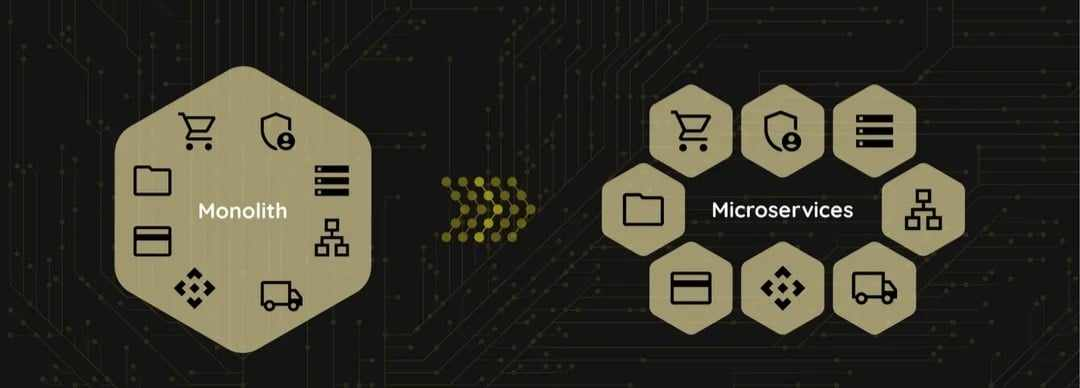
\includegraphics[scale = 0.4]{pictures/anh_khac_nhau_giua_kien_truc_nguyen_khoi_va_kien_truc_vi_dich_vu/main.jpg}

\caption{Ảnh khác nhau giữa kiến trúc nguyên khối và kiến trúc vi dịch vụ}

\end{figure}



% \subsection{Một số đặc điểm và ưu điểm của kiến trúc vi dịch vụ}

% Kiến trúc vi dịch vụ có nhiều ưu điểm, đặc biệt với các dự án có quy mô lớn và phức tạp.

\begin{itemize}

\item Kiến trúc vi dịch vụ phân chia dự án thành các dịch vụ nhỏ.

\begin{itemize}

\item Giúp việc phát triển và quản lý hệ thống dễ dàng hơn.

\item Tận dụng tài nguyên theo nhu cầu cho từng dịch vụ riêng.

\end{itemize}

\item Các dịch vụ độc lập về nghiệp vụ kinh doanh.

Các nhóm không cần hiểu sâu về mọi khía cạnh kinh doanh. Dẫn tới tốc độ phát triển và tốc độ định giá doanh nghiệp nhanh hơn.

\item Các dịch vụ độc lập về ngôn ngữ lập trình và CSDL

Ví dụ: Mỗi dịch vụ sử dụng ngôn ngữ lập trình và CSDL khác nhau như: NodeJS, Go, Python, Java, CSharp, MongoDB, SQLServer, SQLite, MySQL, PostgreSQL

\begin{figure}[H]

\centering

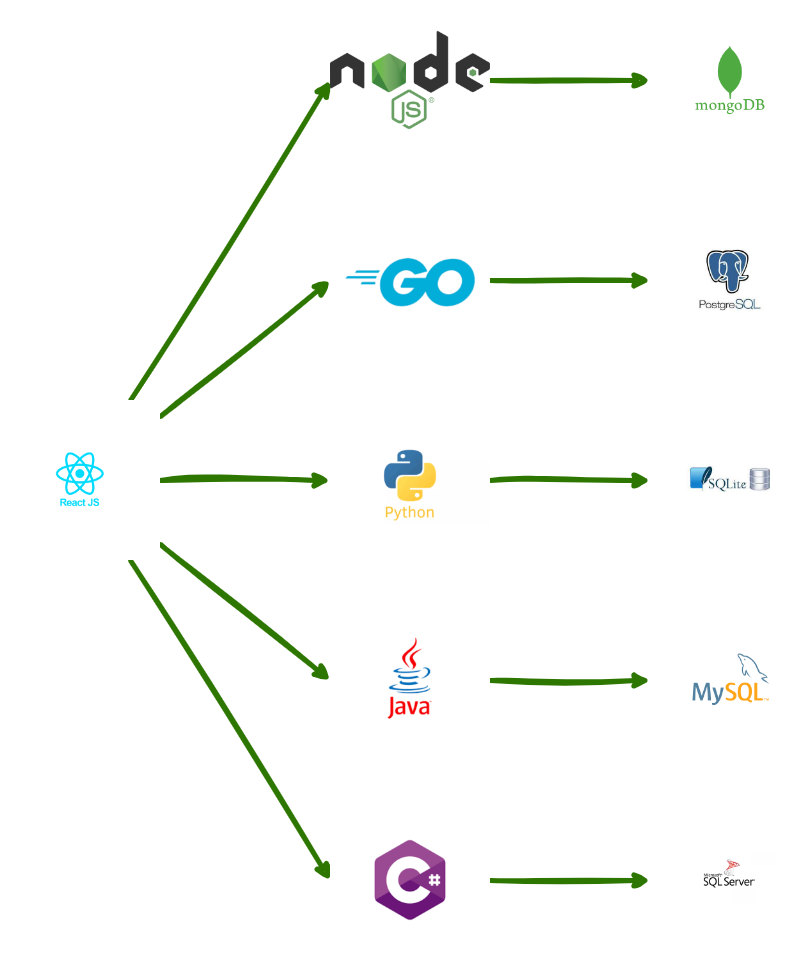
\includegraphics[scale = 0.3]{pictures/da_ngon_ngu_va_csdl/main.drawio.png}
 
\caption{Các dịch vụ độc lập về ngôn ngữ lập trình và CSDL}

\end{figure}

\begin{itemize}

\item Kiến trúc vi dịch vụ sử dụng đa ngôn ngữ và công nghệ khác nhau. Từ đó tận dụng hiệu quả thế mạnh của từng ngôn ngữ, công nghệ phù hợp nhất cho yêu cầu nghiệp vụ cụ thể.

\item Giảm chi phí và thời gian kiểm thử do ít ràng buộc.

\end{itemize}

\item Các dịch vụ độc lập về triển khai hệ thống

Mỗi dịch vụ triển khai độc lập và có thể thay đổi mà không ảnh hưởng đến các dịch vụ khác.

Giảm ràng buộc và tăng tính linh hoạt của hệ thống. Từ đó dễ dàng mở rộng hệ thống.

\item Hệ thống có khả năng chịu lỗi tăng độ tin cậy.

Do các dịch vụ độc lập, nhiều dịch vụ có thể triển khai trong cùng một khả năng kinh doanh để đảm bảo tính sẵn sàng của hệ thống.

\end{itemize}

%%%%%%%%%%%%%%%%%%%%%%%%%%%%%%%%%%%%%

% Các dịch vụ tương tác với nhau qua hạ tầng mạng.



% \newpage

% \newpage

% \newpage

% \newpage

% \newpage

% \newpage

% \newpage

% \newpage

% \newpage

% \newpage

% \newpage

% \newpage

% \newpage

% \subsection{Một số nhược điểm và thách thức của kiến trúc vi dịch vụ}

% Mặc dù kiến trúc vi dịch vụ có nhiều lợi ích, nhưng cũng có nhiều thách thức:

\begin{itemize}

\item Chịu ảnh hưởng của đường truyền mạng.

\item Đồng bộ đồng hồ thời gian.

\item Ràng buộc về thứ tự sự kiện.

\item Tính nhất quán và toàn vẹn của dữ liệu.

\item Khả năng kiểm soát giao dịch.

\item Giám sát giữa các dịch vụ.

\item Bảo mật giao tiếp giữa các dịch vụ.

\item Phát hiện lỗi và sửa lỗi khó khăn, phức tạp hơn.

\item Chi phí xây dựng và quản lý vận hành lớn.

\end{itemize}



%%%%%%%%%%%%%%%%%%%%%%%%%%%%%%%%%%

% \section{Giới thiệu về thiết kế hướng miền}

% Kiến trúc vi dịch vụ giải quyết những thách thức và hỗ trợ doanh nghiệp chuyển đổi kinh doanh, mở rộng hệ thống dễ dàng. Tuy nhiên, để xây dựng được một kiến trúc vi dịch vụ tốt, cần phải tạo ra các dịch vụ nhỏ phù hợp và duy trì tính độc lập. Trong đồ án này, em sử dụng thiết kế hướng miền để phân tích và xây dựng kiến trúc vi dịch vụ. Thiết kế hướng miền giúp xác định và tổ chức các dịch vụ dựa trên việc hiểu rõ về lĩnh vực kinh doanh, từ đó giúp dự án phản ánh chính xác các quy trình và quy tắc kinh doanh.



Thiết kế hướng miền được Eric Evans giới thiệu trong cuốn sách               \textit{"Domain Driven Design: Tackling Complexity in the Heart of Software"}. \emph{Thiết kế hướng miền (Domain Driven Design) }  là một tư tưởng, một hướng tiếp cận   thiết kế phần mềm tập trung vào việc hiểu rõ và mô hình hóa lĩnh vực kinh doanh của một tổ chức.          Thiết kế hướng miền nhấn mạnh việc sử dụng lĩnh vực nghiệp vụ kinh doanh để thảo luận và đề xuất giải pháp đáp ứng nhu cầu. Vì để tạo một phần mềm tốt, chúng ta cần phải hiểu rõ về chính phần mềm đó.

Trong nhiều ứng dụng thường có phần xử lý các công việc không liên quan đến vấn đề nghiệp vụ như truy cập file, hạ tầng mạng, CSDL,... trong đối tượng nghiệp vụ kinh doanh. Cách này giúp tốc độ hoàn thiện ứng dụng nhanh. Tuy nhiên, cách này làm cho thiết kế bị mất đi tính hướng đối tượng trong thực tế với mức độ doanh nghiệp lớn.

Trong kiến trúc vi dịch vụ, thiết kế hướng miền giúp đảm bảo rằng mỗi dịch vụ được thiết kế phản ánh một phần cụ thể của lĩnh vực kinh doanh. Mỗi dịch vụ được quản lí bởi một nhóm nhỏ được hỗ trợ bởi các chuyên gia ngành.


 

Trong thiết kế hướng miền, \emph{chuyên gia ngành (Domain Expert)} là người có kiến thức và hiểu biết sâu sắc về vấn đề đang được hệ thống phần mềm giải quyết. Chuyên gia ngành thể hiện chính xác vấn đề kinh doanh, đóng vai trò là nguồn thông tin cho nhóm phát triển.



% \subsection{Đôi nét về thiết kế hướng miền (Domain Driven Design)}

% Thiết kế hướng miền được Eric Evans giới thiệu trong cuốn sách "Domain Driven Design: Tackling Complexity in the Heart of Software".

Thiết kế hướng miền (Domain Driven Design) là một phương pháp thiết kế phần mềm tập trung vào việc hiểu rõ và mô hình hóa lĩnh vực kinh doanh của một tổ chức.

Thiết kế hướng miền nhấn mạnh việc sử dụng lĩnh vực nghiệp vụ kinh doanh để thảo luận và đề xuất giải pháp đáp ứng nhu cầu. Vì để tạo một phần mềm tốt, chúng ta cần phải hiểu rõ về chính phần mềm đó.

Trong nhiều ứng dụng thường có phần xử lý các công việc không liên quan đến vấn đề nghiệp vụ như truy cập file, hạ tầng mạng, CSDL,... trong đối tượng nghiệp vụ kinh doanh. Cách này giúp tốc độ hoàn thiện ứng dụng nhanh. Tuy nhiên, cách này làm cho thiết kế bị mất đi tính hướng đối tượng trong thực tế với mức độ doanh nghiệp lớn.

Trong kiến trúc vi dịch vụ, thiết kế hướng miền giúp đảm bảo rằng mỗi dịch vụ được thiết kế phản ánh một phần cụ thể của lĩnh vực kinh doanh. Mỗi dịch vụ được quản lí bởi một nhóm nhỏ được hỗ trợ bởi các chuyên gia ngành.



% Trong thiết kế hướng miền, \emph{chuyên gia ngành (Domain Expert)} là người có kiến thức và hiểu biết sâu sắc về vấn đề đang được hệ thống phần mềm giải quyết. Chuyên gia ngành thể hiện chính xác vấn đề kinh doanh, đóng vai trò là nguồn thông tin cho nhóm phát triển.



% \subsection{Định nghĩa miền (Domain)}

% Hệ thống phần mềm được tạo ra để xử lý sự phức tạp trong cuộc sống hiện đại. Việc phát triển hệ thống liên kết chặt chẽ với một số khía cạnh cụ thể trong cuộc sống của chúng ta.

Trong domain driven design, \emph{miền (Domain)} đề cập đến phạm vi kiến thức và vấn đề cụ thể mà hệ thống xử lý.

Xét theo góc độ kinh doanh và góc độ hệ thống:

\begin{itemize}

\item Về góc độ kinh doanh: miền đại diện cho một lĩnh vực hoặc ngành mà doanh nghiệp hoạt động.

\item Về góc độ hệ thống: miền có thể coi là đại diện cho không gian vấn đề của hệ thống.

\end{itemize}

Hệ thống cần phản ánh đúng miền và hiện thực hóa chính xác miền.

\begin{example} \emph{Trong đồ án này, miền được xác định là bài toán giải pháp hóa đơn điện tử.}

\end{example}

% \subsection{Giới thiệu về các mẫu chiến lược và các mẫu kỹ thuật}

% Thiết kế hướng miền cung cấp 2 loại mẫu:

\begin{itemize}

\item \emph{Các mẫu chiến lược (Strategic Patterns):} Phân chia một miền lớn và phức tạp thành các phần nhỏ hơn với ranh giới được xác định rõ ràng. Giúp phân chia một miền lớn hợp lý.

\item \emph{Các mẫu kỹ thuật (Tactical Patterns):} Hiện thực hóa các khái niệm và qui trình trong thành phần thành các thiết kế hệ thống phần mềm. Giúp hệ thống phù hợp với kinh doanh.

\end{itemize}

\begin{figure}[H]

\centering

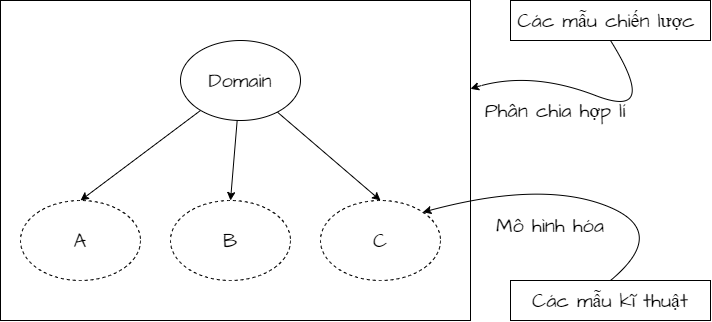
\includegraphics[scale = 0.5]{pictures/cac_mau_chien_luoc_va_cac_mau_ky_thuat/main.drawio.png}

\caption{Tổng quan về Strategic Patterns và Tactical Patterns}

\end{figure}

%%%%%%%%%%%%%%%%%%%%%%%%%%%%%%%%%%
%%%%%%%%%%%%%%%%%%%%%%%%%%%%%%%%%%
%%%%%%%%%%%%%%%%%%%%%%%%%%%%%%%%%%
%%%%%%%%%%%%%%%%%%%%%%%%%%%%%%%%%%
%%%%%%%%%%%%%%%%%%%%%%%%%%%%%%%%%%
%%%%%%%%%%%%%%%%%%%%%%%%%%%%%%%%%%
%%%%%%%%%%%%%%%%%%%%%%%%%%%%%%%%%%
%%%%%%%%%%%%%%%%%%%%%%%%%%%%%%%%%%
%%%%%%%%%%%%%%%%%%%%%%%%%%%%%%%%%%
%%%%%%%%%%%%%%%%%%%%%%%%%%%%%%%%%%
%%%%%%%%%%%%%%%%%%%%%%%%%%%%%%%%%%
%%%%%%%%%%%%%%%%%%%%%%%%%%%%%%%%%%
%%%%%%%%%%%%%%%%%%%%%%%%%%%%%%%%%%
%%%%%%%%%%%%%%%%%%%%%%%%%%%%%%%%%%
%%%%%%%%%%%%%%%%%%%%%%%%%%%%%%%%%%
%%%%%%%%%%%%%%%%%%%%%%%%%%%%%%%%%%
%%%%%%%%%%%%%%%%%%%%%%%%%%%%%%%%%%
%%%%%%%%%%%%%%%%%%%%%%%%%%%%%%%%%%
%%%%%%%%%%%%%%%%%%%%%%%%%%%%%%%%%%

\chapter{Các mẫu chiến lược}

% Các mẫu chiến lược phân tích nghiệp vụ kinh doanh sau đó đưa ra việc phân chia các thành phần và hiểu mối quan hệ của các thành phần đó. Từ đó, các mẫu chiến lược giúp xác định các thành phần quan trọng của hệ thống, đảm bảo kiến trúc phần mềm phản ánh đúng các yêu cầu kinh doanh. Từ việc phân chia hệ thống thành các thành phần nhỏ, chúng ta có thể tạo ra hệ thống mở rộng dễ dàng, phát triển linh hoạt theo nhu cầu kinh doanh.

Các mẫu chiến lược bao gồm:

\begin{itemize}

% các mục nhỏ ben dưới

% các mục nhỏ ben dưới

% các mục nhỏ ben dưới

% các mục nhỏ ben dưới

% các mục nhỏ ben dưới

% các mục nhỏ ben dưới

\item Muc1

\item Muc2

\item Muc1

\item Muc2

\item Muc1

\item Muc2

\item Muc1

\item Muc2

\end{itemize}

% nội dung trang lớn lên để hết giấy

% nội dung trang lớn lên để hết giấy

% nội dung trang lớn lên để hết giấy

% nội dung trang lớn lên để hết giấy

% nội dung trang lớn lên để hết giấy

\begin{figure}[H]

\centering

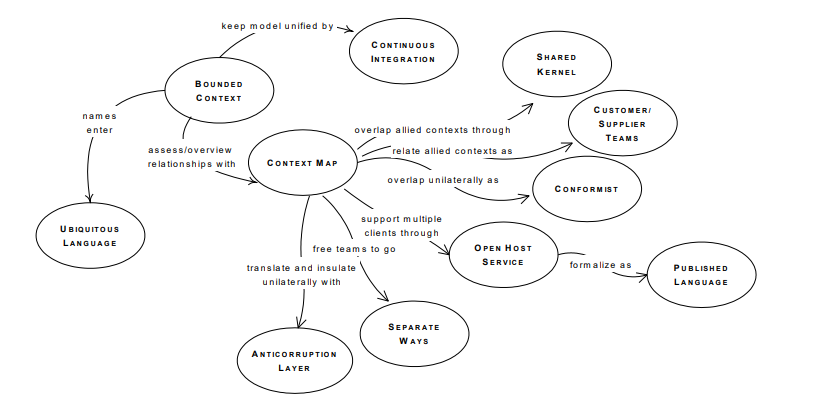
\includegraphics[scale = 0.9]{pictures/cac_mau_chien_luoc/temp.png}

\caption{Sơ đồ về các thành phần trong mô hình chiến lược}

\end{figure}

%!<! - - $ Vẽ lại sau: - - >

%!<! - - $ Vẽ lại sau: - - >

%!<! - - $ Vẽ lại sau: - - >

%!<! - - $ Vẽ lại sau: - - >

%!<! - - $ Vẽ lại sau: - - >

%!<! - - $ Vẽ lại sau: - - >

%!<! - - $ Vẽ lại sau: - - >

%!<! - - $ Vẽ lại sau: - - >

%!<! - - $ Vẽ lại sau: - - >

%!<! - - $ Vẽ lại sau: - - >



% \newpage

% \newpage

% \newpage

% \newpage

% \newpage

% \newpage

% \newpage

% \newpage

% \newpage

% \newpage

% \newpage

% \newpage

% \newpage

% \section{Miền phụ (Sub - Domain)}

% Một miền lớn được tạo thành từ nhiều \emph{miền phụ (Sub - Domain)}. Trong thực tế, một miền kinh doanh phức tạp không thể có một chuyên gia ngành có kiến thức về tất cả các miền phụ.

\begin{example} Trong miền thương mại điện tử lớn có thể có một số miền phụ sau:

\begin{itemize}

\item \textbf{Miền phụ quản lý hàng tồn kho:} liên quan đến việc quản lý sản phẩm trong kho hàng.

\item \textbf{Miền phụ quản lý khách hàng:} liên quan đến việc quản lý tài khoản khách hàng.

\item \textbf{Miền phụ vận chuyển:} liên quan đến việc quản lý việc vận chuyển giao hàng.

\end{itemize}

\end{example}


% \subsection{Phân loại các miền phụ}

% Trong thiết kế hướng miền, có ba loại miền phụ là:

\begin{itemize}

\item Miền phụ chung (Generic Subdomain)

\item Miền phụ cốt lõi (Core Subdomain)

\item Miền phụ hỗ trợ (Supporting Subdomain)

\end{itemize}

% \subsubsection{Miền phụ chung (Generic Subdomain)}

% Miền phụ chung cung cấp các giải pháp có sẵn mà doanh nghiệp có thể mua. Miền phụ chung có thể được tìm thấy trên nhiều ngành. Doanh nghiệp không thể đạt được bất kỳ lợi thế cạnh tranh nào so với đối thủ bằng cách thực hiện những điều khác biệt trong miền phụ chung.

\begin{example} Các miền phụ chung \textit{"quản lý nhân sự"} hay \textit{"quản lý cơ sở vật chất"} không tạo thêm bất kỳ giá trị khác biệt nào cho doanh nghiệp.

\end{example}



% \subsubsection{Miền phụ cốt lõi (Core Subdomain)}

% Miền phụ cốt lõi là phần quan trọng và có giá trị nhất của hệ thống. Miền phụ cốt lõi giúp phân biệt các doanh nghiệp và làm cho các doanh nghiệp có giá trị. Miền phụ cốt lõi tập trung vào mục tiêu và yêu cầu của khách hàng với doanh nghiệp, từ đó quyết định sự thành công của doanh nghiệp. Vì vậy, mỗi doanh nghiệp luôn tìm cách thực hiện những điều khác biệt trong các miền phụ cốt lõi này để đạt được lợi thế so với đối thủ cạnh tranh.

\begin{example} Trong miền thẻ tín dụng, miền phụ cốt lõi có thể là \textit{"phát hành thẻ"} chịu trách nhiệm về quá trình phát hành thẻ tín dụng cho khách hàng. Miền phụ cốt lõi này bao gồm các nhiệm vụ như: thu thập thông tin khách hàng, thực hiện kiểm tra tín dụng, kích hoạt thẻ, \dots

\end{example}

% \subsubsection{Miền phụ hỗ trợ (Supporting Subdomain)}

% \begin{itemize}

\item Các miền phụ cốt lõi phụ thuộc vào các miền phụ hỗ trợ.

\item Miền phụ hỗ trợ cung cấp các dịch vụ để miền phụ cốt lõi hoạt động hiệu quả.

\item Tuy nhiên, miền phụ hỗ trợ không đòi hỏi mức độ phức tạp cao về logic nghiệp vụ.

\begin{example} Trong nhiều phần mềm, miền phụ hỗ trợ \textit{"xác thực người dùng"} OAuth 2.0 của Facebook hoặc Google hỗ trợ cho miền phụ cốt lõi hoạt động hiệu quả.

\end{example}

\end{itemize}

% \newpage

% \newpage

% \newpage

% \newpage

% \newpage

% \newpage

% \newpage

% \newpage

% \newpage

% \newpage

% \newpage

% \newpage

% \newpage

% \newpage

% \newpage

% \newpage

% \newpage

% \newpage

% \subsection{Cách xác định các miền phụ}

% Các miền phụ cốt lõi, hỗ trợ và chung có thể khác nhau đối với các doanh nghiệp hoạt động trong cùng một miền. Vì các miền phụ được xác định tùy theo nhu cầu kinh doanh và bối cảnh cụ thể của mỗi tổ chức.

\paragraph{Mô tả cách xác định các miền phụ}

\begin{enumerate}

\item Bắt đầu bằng cách xem xét nghiệp vụ kinh doanh.

\item Nếu có sẵn giải pháp đã biết thì có khả năng là miền phụ chung. Ngược lại, chúng ta kiểm tra nghiệp vụ kinh doanh đó có thêm giá trị kinh doanh nào hay không?

\item Nếu không có giá trị kinh doanh thì chúng ta kiểm tra xem các miền phụ cốt lõi có phụ thuộc vào miền phụ này hay không? Nếu có thì có khả năng là miền phụ hỗ trợ. Nếu không thì đó là miền phụ chung.

\item Nếu miền phụ có tiềm năng bổ sung một số giá trị kinh doanh thì bước kiểm tra tiếp theo là xem liệu miền doanh nghiệp có độ phức tạp cao hay không?

\item Nếu miền doanh nghiệp không có độ phức tạp cao thì có khả năng là miền phụ hỗ trợ. Ngược lại thì nó có khả năng là miền phụ cốt lõi.

\end{enumerate}

\begin{figure}[h]

\centering

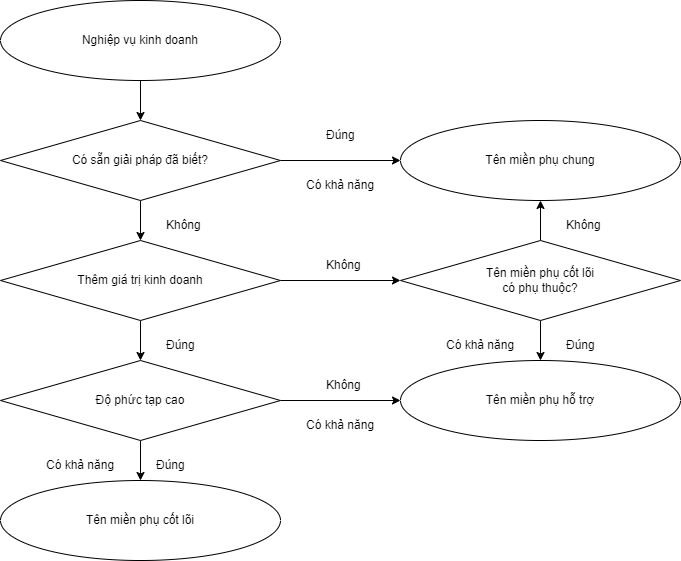
\includegraphics[scale = 0.5]{pictures/cach_xac_dinh_cac_mien_phu/main.drawio.png}

\caption{Sơ đồ xác định các miền phụ}

\end{figure}



% \newpage

% \newpage

% \newpage

% \newpage

% \newpage

% \newpage

% \newpage

% \newpage

% \newpage

% \newpage

% \newpage

% \newpage

% \newpage

% \newpage

% \subsection{Áp dụng phân loại miền phụ trong đồ án này}

% % %!<! - - Hướng dẫn: 5/3 - - >

% %!<! - - Hướng dẫn: 5/3 - - >

% %!<! - - Hướng dẫn: 5/3 - - >

% %!<! - - Hướng dẫn: 5/3 - - >

% %!<! - - Hướng dẫn: 5/3 - - >

% %!<! - - Hướng dẫn: 5/3 - - >

% %!<! - - Hướng dẫn: 5/3 - - >

% %!<! - - Hướng dẫn: 5/3 - - >

% %!<! - - Hướng dẫn: 5/3 - - >

% %!<! - - Hướng dẫn: 5/3 - - >

% %!<! - - Hướng dẫn: 5/3 - - >

% %!<! - - Hướng dẫn: 5/3 - - >

% %!<! - - Hướng dẫn: 5/3 - - >

% %!<! - - Hướng dẫn: 5/3 - - >

% %!<! - - Hướng dẫn: 5/3 - - >

% %!<! - - Hướng dẫn: 5/3 - - >

% ChatGPT?

% Ứng dụng thiết kế hướng miền với hóa đơn điện tử thì miền phụ hỗ trợ có thể là gì?

\subsubsection{Áp dụng phân loại miền phụ trong đồ án này}

\subsubsection{Áp dụng phân loại miền phụ trong đồ án này}

\subsubsection{Áp dụng phân loại miền phụ trong đồ án này}

\subsubsection{Áp dụng phân loại miền phụ trong đồ án này}

\subsubsection{Áp dụng phân loại miền phụ trong đồ án này}

\subsubsection{Áp dụng phân loại miền phụ trong đồ án này}

\subsubsection{Áp dụng phân loại miền phụ trong đồ án này}

\subsubsection{Áp dụng phân loại miền phụ trong đồ án này}

\subsubsection{Áp dụng phân loại miền phụ trong đồ án này}

\subsubsection{Áp dụng phân loại miền phụ trong đồ án này}

\subsubsection{Áp dụng phân loại miền phụ trong đồ án này}

\subsubsection{Áp dụng phân loại miền phụ trong đồ án này}

\subsubsection{Áp dụng phân loại miền phụ trong đồ án này}



% \section{Mô hình miền (Domain Models)}

% Để tạo một phần mềm tốt, chúng ta cần phải hiểu rõ về phần mềm đó. Trong thiết kế hướng miền để có thể hiểu miền nhanh, chúng ta cần tạo ra các mô hình miền. Mô hình miền (Domain Models) là kiến thức có tổ chức và có cấu trúc về miền phù hợp để giải quyết vấn đề kinh doanh. Mục tiêu của mô hình miền là cung cấp rõ ràng, ngắn gọn và chính xác về miền làm cơ sở để hệ thống giải quyết vấn đề kinh doanh.

% \begin{example} Trong đồ án này, mô hình miền của em bao gồm các yêu cầu nghiệp vụ và các sơ đồ: UML Use Case Diagrams, UML Class Diagrams,\dots kĩ thuật ở phần sau

% \end{example}

% \section{Bối cảnh giới hạn (Bounded Context)}

% Một miền cần chia đủ nhỏ để phù hợp với một nhóm cụ thể. Để đạt được điều này, chúng ta cần xác định rõ ranh giới giữa các ngữ cảnh. \emph{Bối cảnh giới hạn (Bounded Context)} giúp xác định rõ các ranh giới, chia miền thành các phần độc lập để giải quyết sự phức tạp trong mô hình doanh nghiệp. Bối cảnh giới hạn tạo ra các mô hình khác nhau cho các lĩnh vực khác nhau của miền. Bối cảnh giới hạn thể hiện phạm vi kinh doanh của dịch vụ.

\begin{figure}[H]

\centering


\includegraphics[scale = 1]{pictures/boi_canh_gioi_han/main.png}

\caption{Ví dụ về bối cảnh giới hạn trong một ngân hàng}

\end{figure}

\subsubsection{Cách xác định bối cảnh giới hạn}

Để có thể xác định được bối cảnh giới hạn chúng ta có thể xem xét:

\begin{itemize}

\item Dựa vào việc phân chia các miền phụ.

\item Dựa vào sơ đồ cấu trúc tổ chức các phòng ban của doanh nghiệp.

\item Dựa vào modules của các ứng dụng kiến trúc nguyên khối (nếu việc phân chia tốt).

\item Dựa vào trách nhiệm và hoạt động của chuyên gia ngành.

\end{itemize}

\subsubsection{Áp dụng xác định bối cảnh giới hạn trong đồ án này}

\subsubsection{Áp dụng xác định bối cảnh giới hạn trong đồ án này}

\subsubsection{Áp dụng xác định bối cảnh giới hạn trong đồ án này}

\subsubsection{Áp dụng xác định bối cảnh giới hạn trong đồ án này}

\subsubsection{Áp dụng xác định bối cảnh giới hạn trong đồ án này}

\subsubsection{Áp dụng xác định bối cảnh giới hạn trong đồ án này}

\subsubsection{Áp dụng xác định bối cảnh giới hạn trong đồ án này}

\subsubsection{Áp dụng xác định bối cảnh giới hạn trong đồ án này}

\subsubsection{Áp dụng xác định bối cảnh giới hạn trong đồ án này}

\subsubsection{Áp dụng xác định bối cảnh giới hạn trong đồ án này}

\subsubsection{Áp dụng xác định bối cảnh giới hạn trong đồ án này}

\subsubsection{Áp dụng xác định bối cảnh giới hạn trong đồ án này}

%!<! - - Hướng dẫn 5/10 - - >

%!<! - - Hướng dẫn 5/10 - - >

%!<! - - Hướng dẫn 5/10 - - >

%!<! - - Hướng dẫn 5/10 - - >

%!<! - - Hướng dẫn 5/10 - - >

%!<! - - Hướng dẫn 5/10 - - >

%!<! - - Hướng dẫn 5/10 - - >

%!<! - - Hướng dẫn 5/10 - - >

%!<! - - Hướng dẫn 5/10 - - >

% \section{Ngôn ngữ chung (Ubiquitous Language)}

% Trong quá trình xây dựng mô hình miền, cần có trao đổi giữa người thiết kế hệ thống và chuyên gia ngành để hiểu đúng về miền. Tuy nhiên, nhóm kinh doanh sử dụng ngôn ngữ kinh doanh và nhóm công nghệ có xu hướng sử dụng các thuật ngữ kỹ thuật trong giao tiếp của họ. Người phát triển phần mềm tập trung vào lớp, phương thức, thuật toán, trong khi chuyên gia ngành thường sử dụng ngôn ngữ chuyên ngành của họ. Sự khác biệt về ngôn ngữ giữa các thành viên có thể dẫn đến những thách thức về giao tiếp. Ngoài ra, trong các lĩnh vực kinh doanh khác nhau, một thuật ngữ có thể được sử dụng trong nhiều miền, cùng với ý nghĩa khác nhau gây ra sự nhầm lẫn và hiểu sai cho các người phát triển phần mềm cũng như các chuyên gia ngành.

Thiết kế hướng miền đề xuất sử dụng ngôn ngữ chung để giải quyết những thách thức ngôn ngữ. \emph{Ngôn ngữ chung (Ubiquitous Language)} là một ngôn ngữ được cấu trúc xung quanh mô hình miền và được tất cả các thành viên trong nhóm sử dụng cho mọi hoạt động của nhóm với phần mềm. Ngôn ngữ chung được xác định bởi các từ vựng và có định nghĩa rõ ràng về ngữ cảnh sử dụng từ vựng.

\subsubsection{Một số đặc điểm của ngôn ngữ chung}

\begin{itemize}

\item Ngôn ngữ chung được sử dụng bởi cả chuyên gia ngành và chuyên gia công nghệ.

\item Có nhiều ngôn ngữ chung trong một tổ chức được mỗi nhóm tạo và quản lý một cách độc lập.

\item Việc tạo ra ngôn ngữ chung là một quá trình liên tục. Ngôn ngữ chung phát triển theo thời gian thông qua sự cộng tác giữa doanh nghiệp và các chuyên gia công nghệ.

\item Các thành viên phải sử dụng ngôn ngữ chung cho công việc và trong toàn bộ hệ thống

\end{itemize}

\begin{figure}[H]

\centering


\includegraphics[scale = 0.6]{pictures/ngon_ngu_chung/main.png}

\caption{Ngôn ngữ chung được sử dụng trong toàn bộ hệ thống}

\end{figure}


%@ Tích hợp liên tục
%@ Tích hợp liên tục
%@ Tích hợp liên tục
%@ Tích hợp liên tục
%@ Tích hợp liên tục
\section{Bản đồ bối cảnh (Context Maps)}
% Các bối cảnh bị giới hạn phải độc lập trong bối cảnh riêng và có mô hình miền riêng, nhưng các bối cảnh bị giới hạn cần tương tác, giao tiếp để trao đổi thông tin. Vì vậy các bối cảnh bị giới hạn có thể có mối quan hệ với nhau. Những mối quan hệ này cần được quản lý chặt chẽ để hoạt động độc lập, nhất quán và linh hoạt. Do đó, cần phải ghi lại các mối quan hệ thông qua việc sử dụng bản đồ bối cảnh. \emph{Bản đồ bối cảnh (Context Maps)} là sự thể hiện trực quan của hệ thống, thể hiện các thành phần và mối quan hệ giữa các thành phần.

\begin{figure}[H]

\centering

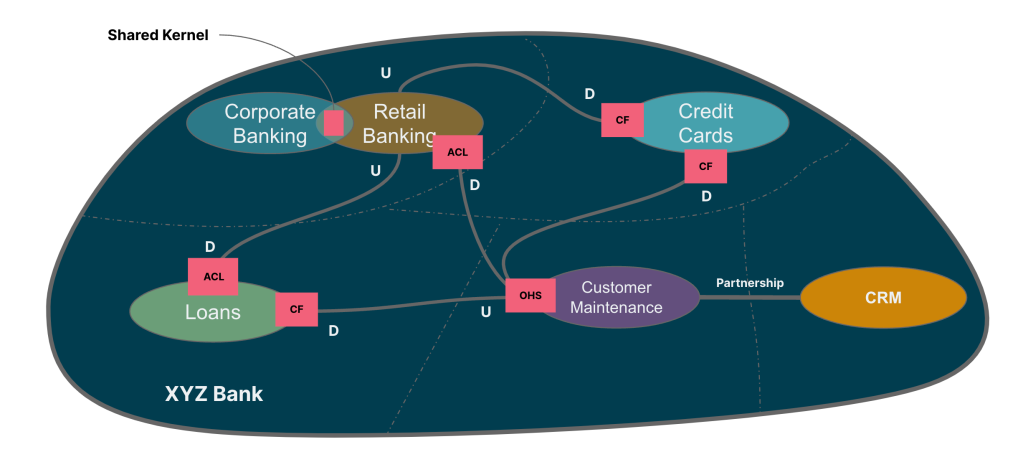
\includegraphics[scale = 0.4]{pictures/ban_do_boi_canh/main.drawio.png}

\caption{Ví dụ bản đồ bối cảnh trong 1 ngân hàng}

\end{figure}

%! Vẽ lại tiếng Việt

%! Vẽ lại tiếng Việt

%! Vẽ lại tiếng Việt

%! Vẽ lại tiếng Việt

%! Vẽ lại tiếng Việt

%! Vẽ lại tiếng Việt

%! Vẽ lại tiếng Việt

%! Vẽ lại tiếng Việt

%! Vẽ lại tiếng Việt

%! Vẽ lại tiếng Việt
\section{Các mối quan hệ bối cảnh giới hạn}
% Có 3 loại mối quan hệ giữa các  bối cảnh bị giới hạn là:

\begin{itemize}

\item Mối quan hệ đối xứng (Symmetric Relationship)

\textbf{Mô tả:} Thể hiện sự tương tác 2 chiều giữa 2 bối cảnh bị giới hạn .

\item Mối quan hệ bất đối xứng (Asymmetric Relationship)

\textbf{Mô tả:} Thể hiện sự tương tác 1 chiều giữa 2 các bối cảnh bị giới hạn .

\item Mối quan hệ 1 - nhiều (One to Many Relationship)

\textbf{Mô tả:} Thể hiện sự tương tác 1 chiều giữa 1 bối cảnh bị giới hạn với nhiều bối cảnh bị giới hạn khác.

\end{itemize}

\begin{figure}[H]

\centering


\includegraphics[scale = 0.5]{pictures/cac_moi_quan_he_boi_canh_gioi_han/main.png}

\caption{Các mối quan hệ bối cảnh bị giới hạn}

\end{figure}



%%%%%%%%%%%%%%%%%%%%%%%%%%%%%%%%%%
%%%%%%%%%%%%%%%%%%%%%%%%%%%%%%%%%%
%%%%%%%%%%%%%%%%%%%%%%%%%%%%%%%%%%
%%%%%%%%%%%%%%%%%%%%%%%%%%%%%%%%%%
%%%%%%%%%%%%%%%%%%%%%%%%%%%%%%%%%%
%%%%%%%%%%%%%%%%%%%%%%%%%%%%%%%%%%
%%%%%%%%%%%%%%%%%%%%%%%%%%%%%%%%%%
% \subsection{Mối quan hệ đối xứng (Symmetric Relationship)}
% \subsubsection{Mô hình riêng biệt (Separate Ways)}
% Mô hình riêng biệt (Separate Ways) khi các bối cảnh bị giới hạn có quan hệ riêng biệt, không có sự phụ thuộc. Vì vậy, các bối cảnh bị giới hạn này có ngôn ngữ, mô hình, mục đích độc lập và thực thi riêng biệt. Các nhóm phát triển không phải cộng tác hay phối hợp với nhau từ đó đem lại lợi ích dễ dàng bảo trì và mở rộng hệ thống.

\begin{example} Trong miền vấn đề ngân hàng, thẻ tín dụng và khoản vay mua nhà không có mối quan hệ.

\begin{figure}[H]

\centering

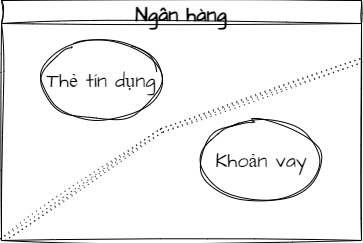
\includegraphics[scale = 0.5]{pictures/mo_hinh_rieng_biet_separate_ways/main.drawio.png}

\caption{Ví dụ mô hình riêng biệt (Separate Ways)}

\end{figure}

\end{example}


% \subsubsection{Mô hình hạt nhân chung (Shared Kernel)}
% Trong thực tế,      nhiều    bối cảnh giới hạn phụ thuộc lẫn nhau.   Mô hình hợp tác (Partnership)   tạo điều kiện     cho việc giao tiếp và cộng tác giữa các       bối cảnh giới hạn phụ thuộc. Tuy nhiên,  sự phụ thuộc     này dẫn đến mức độ kết hợp cao giữa các nhóm và bối cảnh giới hạn,  dẫn tới mất đi tính độc lập. 

\textit{Lưu ý:    Mô hình hợp tác  không phải là mô hình  của  các mẫu chiến lược trong thiết kế huớng miền.}  


Để giải quyết vấn đề   bối cảnh giới hạn phụ thuộc lẫn nhau chúng ta có mô hình      hạt nhân chung.  Mô hình hạt nhân chung (Shared Kernel) cho phép   các    bối cảnh giới hạn  có phần chia sẻ chung  và  có  ranh giới   phân định rõ ràng.  Từ đó, tách việc quản lí các mô hình hạt nhân chung này một cách độc lập với phần còn lại của bối cảnh giới hạn. Khi cần  thay đổi mà không phải của mô hình hạt nhân chung thì nhóm sẽ   hoạt động độc lập.    Thông thường, mô hình hạt nhân chung được hiện thực hóa bằng các thư viện chung.      Tuy nhiên, chỉ sử dụng mô hình hạt nhân chung nếu quan hệ của các   bối cảnh giới hạn   nhỏ và ổn định   để tránh    quan hệ    phức tạp và ràng buộc  chặt chẽ.

% hình ảnh 
% %! $VD: hình giao như 2 tập hợp - - >



% \subsection{Mối quan hệ bất đối xứng (Asymmetric Relationship)}
% % tên gọi chung thượng nguồn, hạ lưu

Trong mối quan hệ bất đối xứng, một bối cảnh giới hạn có sự phụ thuộc vào một bối cảnh giới hạn khác. Mối quan hệ này được mô tả bằng cách gán vai trò cho bối cảnh giới hạn:

Bối cảnh giới hạn thượng nguồn (Upstream): bối cảnh giới hạn cung cấp cho bối cảnh giới hạn khác.

Bối cảnh giới hạn hạ lưu (Downstream): bối cảnh giới hạn phụ thuộc vào bối cảnh giới hạn khác.

%! !ký hiệu: D - U - - >

%! $VD: - - >

%! $VD: A Downstream (D) - B Upstream (U) - - >

%! $VD: Bối cảnh A ràng buộc với bối cảnh B thì: - - >

%! $VD: Bối cảnh A đóng vai trò là bối cảnh giới hạn hạ lưu (Downstream) - - >

%! $VD: Bối cảnh B đóng vai trò là bối cảnh giới hạn thượng nguồn (Upstream) - - >

%! $VD: Bối cảnh giới hạn A có kiến thức về các mô hình trong bối cảnh giới hạn B - - >

%! $VD: Bối cảnh B không có bất kỳ kiến thức nào về mô hình trong bối cảnh giới hạn A - - >


% \subsubsection{Mô hình khách hàng - nhà cung cấp (Customer - Supplier)}
% %! @ - - >

Trong trường hợp bối cảnh giới hạn thượng nguồn đáp ứng nhu cầu của bối cảnh giới hạn hạ lưu.

Trong thực tế khi phát triển, nhóm nhà cung cấp luôn tham khảo ý kiến của nhóm khách hàng để đảm bảo rằng dịch vụ của nhóm nhà cung cấp đáp ứng được nhu cầu của nhóm khách hàng.

% %! Customer/Supplier : https:// thiết kế hướng miền - practitioners.com/customer - supplier

% %! Customer/Supplier : https:// thiết kế hướng miền - practitioners.com/customer - supplier

Trang chủTrang chủBảng chú giảiBối cảnh giới hạn Mối quan hệ bối cảnh giới hạn Nhà cung cấp khách hàng

Nhà cung cấp khách hàng

Mối quan hệ khách hàng - nhà cung cấp là một mối quan hệ bối cảnh giới hạn trong đó một bối cảnh giới hạn phụ thuộc vào một bối cảnh khác về chức năng hoặc dữ liệu của nó. Bối cảnh giới hạn phụ thuộc được gọi là khách hàng, trong khi bối cảnh độc lập được gọi là nhà cung cấp. Khách hàng đưa ra yêu cầu với nhà cung cấp và nhà cung cấp sẽ đưa ra phản hồi để thực hiện các yêu cầu đó.

Mối quan hệ khách hàng - nhà cung cấp thường được sử dụng khi một bối cảnh giới hạn yêu cầu thông tin hoặc chức năng từ một bối cảnh giới hạn khác. Bằng cách thiết lập sự phụ thuộc rõ ràng giữa hai bối cảnh, các thay đổi có thể được thực hiện đối với một bối cảnh mà không ảnh hưởng đến bối cảnh kia, miễn là giao diện giữa chúng vẫn ổn định. Điều này cho phép tính mô - đun hóa và tính linh hoạt cao hơn trong kiến trúc hệ thống tổng thể.

Hàm ý

Mối quan hệ khách hàng - nhà cung cấp giữa các bối cảnh giới hạn có những ưu và nhược điểm sau:

Ưu điểm

Phân tách rõ ràng mối quan tâm giữa hai bối cảnh giới hạn

Có thể tạo điều kiện cho việc mô - đun hóa và đóng gói chức năng

Bối cảnh nhà cung cấp có thể tập trung vào việc cung cấp một dịch vụ hoặc chức năng cụ thể cho bối cảnh khách hàng

Bối cảnh khách hàng có thể dựa vào bối cảnh nhà cung cấp để có chức năng cụ thể mà không cần hiểu chi tiết triển khai

Nhược điểm

Sự liên kết chặt chẽ giữa hai bối cảnh, điều này có thể gây khó khăn cho việc thay đổi một bối cảnh mà không ảnh hưởng đến bối cảnh kia

Có thể dẫn đến sự phổ biến của API và sự phụ thuộc giữa hai bối cảnh

Yêu cầu quản lý cẩn thận giao diện và hợp đồng giữa hai bối cảnh để đảm bảo rằng chúng vẫn tương thích

Có thể dẫn đến sự thiếu hợp tác và giao tiếp giữa các nhóm chịu trách nhiệm về hai bối cảnh, điều này có thể cản trở tiến trình và sự hiểu biết chung

Nhìn chung, mối quan hệ khách hàng - nhà cung cấp có thể hữu ích trong một số trường hợp nhất định, nhưng nó đòi hỏi sự quản lý và giao tiếp cẩn thận để đảm bảo rằng hai bối cảnh vẫn tương thích và những thay đổi trong bối cảnh này không gây ra hậu quả ngoài ý muốn cho bối cảnh kia.

Ví dụ

Hãy xem xét một ứng dụng thương mại điện tử nơi khách hàng có thể đặt hàng và hệ thống cần quản lý việc tồn kho sản phẩm. Trong trường hợp này, chúng ta có thể có hai bối cảnh giới hạn :

Bối cảnh giới hạn quản lý đơn hàng: Bối cảnh này quản lý tất cả các hoạt động liên quan đến đơn hàng như đặt hàng, quản lý lịch sử đơn hàng, quản lý trạng thái vận chuyển và giao hàng, v.v. Bối cảnh này có vai trò khách hàng vì nó tương tác trực tiếp với khách hàng.

Bối cảnh giới hạn quản lý hàng tồn kho: Bối cảnh này quản lý việc kiểm kê sản phẩm như thêm và xóa sản phẩm, theo dõi mức tồn kho của sản phẩm và thông báo khi mức tồn kho thấp. Ngữ cảnh này có vai trò nhà cung cấp vì nó cung cấp dữ liệu tồn kho cần thiết cho Ngữ cảnh giới hạn quản lý đơn hàng.

Trong ví dụ này, chúng ta có thể thấy rằng Bối cảnh giới hạn quản lý hàng tồn kho đang đóng vai trò là nhà cung cấp cho Bối cảnh giới hạn quản lý đơn hàng đang đóng vai trò là khách hàng. Bối cảnh giới hạn quản lý hàng tồn kho cung cấp thông tin cần thiết cho Bối cảnh giới hạn quản lý đơn hàng để đảm bảo rằng mức tồn kho được cập nhật chính xác và đơn hàng có thể được thực hiện.

Điểm mấu chốt cần lưu ý ở đây là hai bối cảnh giới hạn có vai trò và trách nhiệm được xác định rõ ràng. Bối cảnh giới hạn quản lý đơn hàng dựa trên Bối cảnh giới hạn quản lý hàng tồn kho cho dữ liệu liên quan đến hàng tồn kho và Bối cảnh giới hạn quản lý hàng tồn kho chịu trách nhiệm duy trì và cập nhật dữ liệu hàng tồn kho.

Khi nào nó hoạt động?

Mối quan hệ khách hàng - nhà cung cấp có thể hoạt động hiệu quả trong các tình huống sau:

Giao diện được xác định rõ ràng: Khi giao diện giữa các bối cảnh được giới hạn được xác định rõ ràng, việc thiết lập mối quan hệ khách hàng - nhà cung cấp rõ ràng sẽ dễ dàng hơn.

Trách nhiệm rõ ràng: Khi khách hàng và nhà cung cấp có trách nhiệm rõ ràng, việc đảm bảo rằng mỗi bối cảnh được tập trung vào miền riêng của nó sẽ dễ dàng hơn và có thể được phát triển độc lập.

Sự phụ thuộc hạn chế: Khi mối quan hệ khách hàng - nhà cung cấp có sự phụ thuộc hạn chế, nó sẽ giảm nguy cơ kết hợp giữa các bối cảnh.

Giao tiếp mạnh mẽ: Khi khách hàng và nhà cung cấp giao tiếp hiệu quả và thường xuyên, điều đó sẽ giúp thiết lập mối quan hệ hợp tác và hiệu quả.

Tầm nhìn chung: Khi khách hàng và nhà cung cấp chia sẻ tầm nhìn và mục tiêu chung, điều đó sẽ tạo điều kiện cho sự hợp tác và giúp mối quan hệ hợp tác hiệu quả hơn.

Khi nào nó không hoạt động?

Mối quan hệ khách hàng - nhà cung cấp trong thiết kế hướng miền có thể không hoạt động trong một số trường hợp nhất định như:

Sự kết hợp chặt chẽ: Nếu bối cảnh của khách hàng và nhà cung cấp trở nên gắn kết chặt chẽ với nhau, thì bất kỳ thay đổi nào trong một bối cảnh đều có thể yêu cầu những thay đổi trong bối cảnh kia, điều này làm mất đi mục đích xác định các bối cảnh giới hạn độc lập.

Mục tiêu kinh doanh không phù hợp: Nếu mục tiêu kinh doanh của bối cảnh khách hàng và nhà cung cấp không thống nhất, điều đó có thể dẫn đến xung đột và khó khăn trong việc xác định giao diện và hợp đồng.

Giao tiếp không đầy đủ: Giao tiếp hiệu quả là rất quan trọng để đảm bảo rằng bối cảnh của khách hàng và nhà cung cấp hiểu được nhu cầu và yêu cầu của nhau. Giao tiếp không đầy đủ có thể dẫn đến hiểu lầm và dẫn đến các giao diện và hợp đồng được xác định kém.

Quá phụ thuộc vào bối cảnh của nhà cung cấp: Nếu bối cảnh của khách hàng trở nên quá phụ thuộc vào bối cảnh của nhà cung cấp, điều đó có thể gây ra vấn đề nếu bối cảnh của nhà cung cấp không thành công hoặc thay đổi theo cách không đáp ứng được nhu cầu của khách hàng.

Thiếu kiến thức chuyên môn về miền: Nếu bối cảnh khách hàng thiếu kiến thức chuyên môn về miền và phụ thuộc nhiều vào bối cảnh của nhà cung cấp để được hướng dẫn, điều đó có thể dẫn đến các giao diện và hợp đồng được xác định kém.

% %! Customer/Supplier : https:// thiết kế hướng miền - practitioners.com/customer - supplier

% %! Customer/Supplier : https:// thiết kế hướng miền - practitioners.com/customer - supplier

% %! Customer/Supplier : https:// thiết kế hướng miền - practitioners.com/customer - supplier

% %! Customer/Supplier : https:// thiết kế hướng miền - practitioners.com/customer - supplier

% Khách hàng - Nhà cung cấp : Đây là mối quan hệ trong đó một bối cảnh giới hạn cung cấp dịch vụ hoặc dữ liệu cho bối cảnh khác. Bối cảnh khách hàng dựa vào bối cảnh nhà cung cấp để có những khả năng hoặc dữ liệu nhất định. Những thay đổi trong bối cảnh nhà cung cấp có thể tác động đến bối cảnh khách hàng, vì vậy điều quan trọng là phải quản lý mối quan hệ này một cách cẩn thận.
% \subsubsection{Mô hình tuân thủ (Conformist)}
% Mô hình tuân thủ là một mối quan hệ trong đó bối cảnh giới hạn hạ lưu áp dụng mô hình, ngôn ngữ chung và các khái niệm được sử dụng bởi bối cảnh giới hạn thượng nguồn.

Cả hai bối cảnh giới hạn đều sử dụng cùng một mô hình. Vì vậy, chúng ta không cần dịch mô hình giữa các bối cảnh giới hạn.

%!! ký hiệu: CF - U - - >

%! $VD: - - >

%! $VD: A - CF - U - B - - >

%! $VD: A - users(id, name) - B cũng users(id, name) - - >

% %! Conformist : https:// thiết kế hướng miền - practitioners.com/conformist

% %! Conformist : https:// thiết kế hướng miền - practitioners.com/conformist

% %! Conformist : https:// thiết kế hướng miền - practitioners.com/conformist

% %! Conformist : https:// thiết kế hướng miền - practitioners.com/conformist

% %! Conformist : https:// thiết kế hướng miền - practitioners.com/conformist

Trang chủTrang chủBảng chú giảiBối cảnh giới hạn Mối quan hệ bối cảnh giới hạn người theo chủ nghĩa tuân thủ

người theo chủ nghĩa tuân thủ

Mối quan hệ tuân thủ giữa các ngữ cảnh giới hạn đề cập đến mối quan hệ trong đó một ngữ cảnh giới hạn tuân theo cùng một ngôn ngữ chung và cùng các khái niệm được sử dụng bởi một ngữ cảnh khác bối cảnh giới hạn . Nói cách khác, bối cảnh giới hạn tuân thủ áp dụng mô hình, ngôn ngữ và hành vi của bối cảnh giới hạn khác.

Mối quan hệ này được thiết lập khi một bối cảnh giới hạn là chủ sở hữu rõ ràng của một khái niệm hoặc mô hình miền cụ thể và một bối cảnh giới hạn khác cần tương tác với nó hoặc sử dụng các dịch vụ của nó. Bối cảnh giới hạn tuân thủ cần phải tuân thủ các điều khoản và khái niệm của bối cảnh giới hạn chủ sở hữu để đảm bảo sự tương tác suôn sẻ giữa chúng.

Mối quan hệ tuân thủ là một trong những mối quan hệ ít phổ biến hơn giữa các bối cảnh giới hạn và thường chỉ được thiết lập trong những trường hợp rất cụ thể trong đó hai hoặc nhiều bối cảnh giới hạn chia sẻ các miền rất gần nhau, chẳng hạn như trong trường hợp các vi dịch vụ cần giao tiếp với nhau.

Hàm ý

Mối quan hệ tuân thủ giữa các bối cảnh giới hạn trong thiết kế hướng miền có nghĩa là một bối cảnh giới hạn tuân theo mô hình của bối cảnh giới hạn khác và mọi thay đổi đối với mô hình tuân thủ phải tuân theo mô hình của nhà cung cấp.

Ưu điểm

Giảm độ phức tạp: Bởi vì bối cảnh giới hạn tuân thủ được mô hình hóa theo bối cảnh giới hạn của nhà cung cấp, nên không cần phải xử lý các mô hình khác nhau và hai bối cảnh có thể hoạt động liền mạch với nhau.

Tích hợp dễ dàng: Vì bối cảnh giới hạn tuân thủ được mô hình hóa theo bối cảnh giới hạn của nhà cung cấp, nên rất dễ tích hợp hai bối cảnh với nhau.

Nhược điểm

Mất quyền tự chủ: Bối cảnh giới hạn tuân thủ không thể phát triển độc lập với bối cảnh giới hạn nhà cung cấp và mọi thay đổi đối với mô hình bối cảnh giới hạn nhà cung cấp sẽ cần phải được phản ánh trong mô hình bối cảnh giới hạn tuân thủ.

Sự phụ thuộc vào bối cảnh giới hạn của nhà cung cấp: Bối cảnh giới hạn của nhà cung cấp phụ thuộc rất nhiều vào bối cảnh giới hạn của nhà cung cấp và bất kỳ thay đổi nào đối với bối cảnh giới hạn của nhà cung cấp đều có thể có tác động đáng kể đến bối cảnh giới hạn của nhà cung cấp.

Các vấn đề về hiệu suất có thể xảy ra: Bối cảnh giới hạn tuân thủ có thể phải thực hiện các chuyển đổi hoặc chuyển đổi bổ sung để phù hợp với mô hình bối cảnh giới hạn của nhà cung cấp, điều này có thể ảnh hưởng đến hiệu suất.

Nhìn chung, mối quan hệ tuân thủ có thể hữu ích trong các tình huống trong đó bối cảnh giới hạn của nhà cung cấp có tính ổn định cao và khó có thể thay đổi, đồng thời khi bối cảnh giới hạn tuân thủ yêu cầu mức độ tích hợp cao với bối cảnh giới hạn của nhà cung cấp.

Ví dụ

Dưới đây là ví dụ về mối quan hệ tuân thủ giữa hai bối cảnh giới hạn trong một ứng dụng thương mại điện tử giả định:

Một bối cảnh giới hạn chịu trách nhiệm xử lý các đơn đặt hàng và thanh toán, trong khi một bối cảnh giới hạn khác chịu trách nhiệm quản lý hàng tồn kho. Trong trường hợp này, bối cảnh giới hạn khoảng không quảng cáo sẽ là người tuân thủ và bối cảnh giới hạn đơn hàng và thanh toán sẽ là khách hàng.

Bối cảnh giới hạn khoảng không quảng cáo sẽ cung cấp một giao diện được tiêu chuẩn hóa mà bối cảnh giới hạn đơn đặt hàng và thanh toán có thể sử dụng để truy vấn mức tồn kho và cập nhật số lượng khoảng không quảng cáo. Bối cảnh đặt hàng và thanh toán sẽ tuân theo giao diện này, đảm bảo rằng mọi cập nhật mà nó thực hiện đối với số lượng hàng tồn kho đều được thực hiện theo cách mong đợi.

Ví dụ: ngữ cảnh đơn đặt hàng và thanh toán có thể sử dụng API sau để đặt trước hàng tồn kho khi đặt hàng:

1

<code>inventory.reserve(productId, quantity);

Bối cảnh giới hạn khoảng không quảng cáo sẽ xác định API này và bối cảnh giới hạn đơn đặt hàng và thanh toán sẽ tuân theo API đó. Điều này cho phép hai bối cảnh hoạt động liền mạch với nhau, mặc dù chúng tách biệt và độc lập.

Khi nào nó hoạt động?

Mối quan hệ tuân thủ giữa các bối cảnh giới hạn hoạt động hiệu quả trong các trường hợp sau:

Khi có bối cảnh rõ ràng và chi phối: Bối cảnh giới hạn tuân thủ phải ít phức tạp hơn và ít quan trọng hơn bối cảnh giới hạn chi phối.

Khi bối cảnh tuân thủ có thể chấp nhận những thay đổi: Bối cảnh tuân thủ phải được thiết kế để thích ứng với những thay đổi do bối cảnh thống trị thực hiện.

Khi có ranh giới rõ ràng: Hai bối cảnh phải có ranh giới rõ ràng và khác biệt.

Khi có mối quan hệ ổn định và vững chắc giữa hai bối cảnh: Cả hai bối cảnh cần hiểu rõ trách nhiệm và vai trò của nhau.

Khi bối cảnh tuân thủ có thể cung cấp giá trị cho bối cảnh thống trị: Bối cảnh tuân thủ phải có thể cung cấp thứ gì đó có giá trị cho bối cảnh thống trị.

Khi nào nó không hoạt động?

Mối quan hệ tuân thủ giữa các bối cảnh giới hạn có thể không hoạt động trong các tình huống sau:

Khi bối cảnh giới hạn tuân thủ trở nên quá phức tạp, gây khó khăn cho việc duy trì sự phân tách rõ ràng các mối quan tâm.

Khi có nhu cầu thay đổi thường xuyên trong bối cảnh giới hạn tuân thủ nhưng lại phụ thuộc vào các bối cảnh giới hạn khác nên không yêu cầu thay đổi.

Khi bối cảnh giới hạn tuân thủ được kết hợp quá chặt chẽ với các bối cảnh giới hạn khác, điều này có thể dẫn đến những hậu quả không lường trước được nếu thực hiện thay đổi.

Khi bối cảnh giới hạn tuân thủ được kết nối quá lỏng lẻo với các bối cảnh giới hạn khác, điều này có thể dẫn đến sự thiếu phối hợp và gắn kết trên toàn hệ thống.

Nói chung, mối quan hệ tuân thủ hoạt động tốt nhất khi sự phụ thuộc giữa các bối cảnh giới hạn tương đối đơn giản và ổn định theo thời gian cũng như khi có sự hiểu biết và thỏa thuận rõ ràng giữa các nhóm chịu trách nhiệm về từng bối cảnh giới hạn .

% %! Conformist : https:// thiết kế hướng miền - practitioners.com/conformist

% %! Conformist : https:// thiết kế hướng miền - practitioners.com/conformist

% %! Conformist : https:// thiết kế hướng miền - practitioners.com/conformist

% %! Conformist : https:// thiết kế hướng miền - practitioners.com/conformist

% Người theo chủ nghĩa tuân thủ : Mối quan hệ này tồn tại khi một bối cảnh giới hạn tuân theo cùng một ngôn ngữ và khái niệm phổ biến như một bối cảnh giới hạn khác. Điều này đảm bảo rằng giao tiếp giữa hai bối cảnh là rõ ràng và rõ ràng.
% \subsubsection{Mô hình chống đổ vỡ (Anti Corruption Layer)}
% bối cảnh giới hạn xuôi dòng quyết định không tuân theo bối cảnh giới hạn ngược dòng.

quyết định tạo ra mô hình của riêng mình thay vì áp dụng các mô hình cho ngữ cảnh giới hạn .

%! Trong trường hợp đó, các mô hình từ ngữ cảnh giới hạn sẽ được hiển thị trong ngữ cảnh giới hạn . Nó sẽ yêu cầu một số loại bản dịch để chuyển đổi các mô hình từ bối cảnh giới hạn sang bối cảnh giới hạn . - - >

%! Đề xuất là tách logic dịch thuật này thành một lớp riêng biệt. Cấp độ này của bản dịch được gọi là trực tiếp chống đổ vỡ - - >

%! Ý tưởng đằng sau luật sư chống đổ vỡ là bảo vệ bối cảnh ngoại quan khỏi tham nhũng. - - >

%!! ký hiệu: ACL - U - - >

trong mỗi bối cảnh liên kết này, có mô hình riêng. Họ không có kiến thức gì về mô hình của nhau.

ACL có kiến thức cần thiết về cả hai mô hình của A và B và thực hiện việc chuyển đổi từ B sang mô hình của A là lớp chống đổ vỡ cần phải có kiến thức về cả mô hình hạ nguồn cũng như mô hình thượng nguồn.

Nhưng hạ lưu không có kiến thức về bối cảnh giới hạn thượng nguồn, và đó là cách lớp chống đổ vỡ bảo vệ hạ lưu khỏi những thay đổi ở thượng nguồn.

%! @ = = = = = = = = = = = = = = = = = = = = = = = - - >

%! Không xem xét kịch bản trong đó bối cảnh giới hạn xuôi dòng quyết định không tuân theo bối cảnh giới hạn ngược dòng. - - >

%! Nói cách khác, nhóm dành cho bối cảnh giới hạn . Nó quyết định tạo ra mô hình của riêng mình thay vì áp dụng các mô hình cho ngữ cảnh giới hạn . - - >

%! Trong trường hợp đó, các mô hình từ ngữ cảnh giới hạn sẽ được hiển thị trong ngữ cảnh giới hạn . Nó sẽ yêu cầu một số loại bản dịch để chuyển đổi các mô hình từ bối cảnh giới hạn sang bối cảnh giới hạn . - - >

%! Đề xuất là tách logic dịch thuật này thành một lớp riêng biệt. Cấp độ này của bản dịch được gọi là trực tiếp chống đổ vỡ và mô hình này còn được gọi là Antichrist. - - >

%! Ý tưởng đằng sau luật sư chống đổ vỡ là bảo vệ bối cảnh ngoại quan khỏi tham nhũng. Loại mối quan hệ này được mô tả bằng cách thay thế ACL. - - >

%! Vì vậy, ở đây chúng tôi đang mô tả mối quan hệ giữa A và B trong mỗi bối cảnh liên kết này, có mô hình riêng. - - >

%! Họ không có kiến thức gì về mô hình của nhau ngoại trừ việc ACL có kiến thức cần thiết về cả hai mô hình của A và B và thực hiện việc chuyển đổi từ morou của B sang mô hình của anh ta. - - >

Và điều này có nghĩa là ánh xạ các thuộc tính khác nhau,

Vì vậy, điều đó có nghĩa là lớp chống đổ vỡ cần phải có kiến thức về cả mô hình hạ nguồn cũng như mô hình thượng nguồn.

Nhưng hạ lưu không có kiến thức về bối cảnh giới hạn thượng nguồn, và đó là cách lớp chống đổ vỡ bảo vệ hạ lưu khỏi những thay đổi ở thượng nguồn.

%!! Lớp chống đổ vỡ này có logic để dịch các mô hình từ định dạng ngược dòng sang định dạng xuôi dòng. - - >

%!!, theo hướng đó xuôi dòng. Bối cảnh giới hạn không có kiến thức về bối cảnh mô hình ngược dòng và do đó không có sự phụ thuộc trực tiếp. - - >

%! @ = = = = = = = = = = = = = = = = = = = = = = = - - >

% %! Anti - Corruption Layer (ACL) : https:// thiết kế hướng miền - practitioners.com/anticorruption - layer

% %! Anti - Corruption Layer (ACL) : https:// thiết kế hướng miền - practitioners.com/anticorruption - layer

% %! Anti - Corruption Layer (ACL) : https:// thiết kế hướng miền - practitioners.com/anticorruption - layer

Trang chủTrang chủBảng chú giảiBối cảnh giới hạn Mối quan hệ bối cảnh giới hạn Lớp chống đổ vỡ

Lớp chống đổ vỡ

Lớp chống đổ vỡ mối quan hệ đề cập đến một mẫu thiết kế trong đó lớp trung gian được tạo giữa hai bối cảnh giới hạn để tạo điều kiện giao tiếp giữa chúng. Lớp chống đổ vỡ đóng vai trò là cầu nối giữa hai miền khác nhau và đảm bảo rằng mỗi ngữ cảnh giới hạn có thể duy trì ngôn ngữ và thuật ngữ riêng mà không bị ảnh hưởng bởi ngữ cảnh kia.

Lớp chống đổ vỡ cung cấp một lớp dịch ánh xạ dữ liệu giữa hai bối cảnh và thực thi các ranh giới giữa chúng. Nó hoạt động như một bộ lọc để đảm bảo rằng ảnh hưởng sai lệch của bối cảnh này không ảnh hưởng đến bối cảnh kia. Mối quan hệ này hữu ích khi có nhu cầu tích hợp với các hệ thống cũ hoặc hệ thống bên ngoài sử dụng các thuật ngữ, công nghệ hoặc cấu trúc dữ liệu khác nhau.

Mục tiêu của mối quan hệ lớp chống đổ vỡ là bảo vệ tính toàn vẹn và quyền tự chủ của từng bối cảnh giới hạn trong khi vẫn cho phép chúng hoạt động cùng nhau một cách hiệu quả.

Hàm ý

Mối quan hệ lớp chống đổ vỡ giữa các bối cảnh giới hạn có những ưu và nhược điểm sau:

Ưu điểm

Cho phép tích hợp các hệ thống cũ với các hệ thống hiện đại bằng cách sử dụng lớp dịch mà không ảnh hưởng đến mô hình miền của hệ thống mới.

Giúp đảm bảo tính toàn vẹn của mô hình miền được duy trì trong hệ thống mới bằng cách cách ly mọi hệ thống cũ có thể không tuân thủ mô hình miền của hệ thống mới.

Khuyến khích phát triển sự tách biệt rõ ràng các mối quan tâm giữa hệ thống mới và hệ thống cũ.

Nhược điểm

Yêu cầu nỗ lực phát triển bổ sung để xây dựng và duy trì lớp chống đổ vỡ .

Có thể tăng thêm độ phức tạp cho kiến trúc hệ thống tổng thể.

Có thể tạo thêm các điểm lỗi trong hệ thống nếu lớp chống đổ vỡ không được triển khai chính xác.

Nhìn chung, việc sử dụng lớp chống đổ vỡ có thể là một công cụ có giá trị để tích hợp các hệ thống cũ với các hệ thống hiện đại theo cách duy trì tính toàn vẹn của mô hình miền và khuyến khích phân tách các mối quan ngại, nhưng nó đòi hỏi phải xem xét cẩn thận về nỗ lực phát triển bổ sung và độ phức tạp tiềm ẩn có thể xảy ra. giới thiệu.

Ví dụ

Giả sử chúng ta có hai bối cảnh giới hạn: một hệ thống cũ xử lý thông tin khách hàng và một hệ thống hiện đại mới cần sử dụng thông tin khách hàng đó. Hệ thống cũ sử dụng lược đồ CSDL riêng và các quy ước đặt tên không tương thích với hệ thống hiện đại. Chúng tôi có thể giới thiệu một lớp chống đổ vỡ giữa hai bối cảnh để chuyển dữ liệu từ hệ thống cũ sang định dạng mà hệ thống hiện đại có thể sử dụng.

Lớp chống đổ vỡ sẽ chịu trách nhiệm:

Hiểu mô hình dữ liệu của hệ thống cũ và nó khác với hệ thống hiện đại như thế nào

Dịch dữ liệu từ định dạng của hệ thống cũ sang định dạng của hệ thống hiện đại

Hiển thị giao diện rõ ràng và nhất quán cho hệ thống hiện đại giúp bảo vệ hệ thống khỏi sự phức tạp của hệ thống cũ

Khi nào nó hoạt động?

Mối quan hệ lớp chống đổ vỡ có hiệu quả trong các trường hợp sau:

Khi nhiều ngữ cảnh giới hạn có mô hình miền và ngôn ngữ riêng và cần giao tiếp với nhau. Trong trường hợp này, lớp chống đổ vỡ đóng vai trò là cầu nối giữa hai ngữ cảnh, dịch mô hình miền và ngôn ngữ của ngữ cảnh này sang ngữ cảnh khác.

Khi một ngữ cảnh giới hạn cần tương tác với một hệ thống cũ có mô hình miền và ngôn ngữ khác. Trong trường hợp này, lớp chống đổ vỡ có thể được sử dụng để dịch mô hình miền và ngôn ngữ của hệ thống cũ sang mô hình miền và ngôn ngữ của ngữ cảnh giới hạn .

Khi một ngữ cảnh giới hạn cần tương tác với một hệ thống hoặc API bên ngoài có mô hình miền và ngôn ngữ khác. Trong trường hợp này, lớp chống đổ vỡ có thể được sử dụng để dịch mô hình miền và ngôn ngữ của hệ thống bên ngoài sang mô hình và ngôn ngữ miền của ngữ cảnh giới hạn .

Nhìn chung, mối quan hệ lớp chống đổ vỡ có hiệu quả khi có nhu cầu tách rời các bối cảnh hoặc hệ thống giới hạn khác nhau có mô hình miền và ngôn ngữ riêng, đồng thời ngăn chặn sự lây nhiễm mô hình miền của bối cảnh giới hạn bởi mô hình miền của bối cảnh hoặc hệ thống khác.

Khi nào nó không hoạt động?

Mối quan hệ lớp chống đổ vỡ giữa các bối cảnh giới hạn là một công cụ mạnh mẽ để giữ cho các bối cảnh giới hạn trở nên độc lập, nhưng nó đi kèm với một số sự đánh đổi. Một sự cân bằng lớn là sự phức tạp và chi phí bổ sung khi triển khai và duy trì lớp chống đổ vỡ . Ngoài ra, nếu lớp chống đổ vỡ không được thiết kế chính xác hoặc nếu nó không được cập nhật với những thay đổi trong bối cảnh giới hạn mà nó đang bảo vệ, thì nó có thể trở thành nút cổ chai hoặc nguồn gây ra lỗi.

Mối quan hệ của lớp chống đổ vỡ hoạt động hiệu quả nhất khi có nhu cầu rõ ràng và khi nó được thiết kế và triển khai chính xác. Nó đặc biệt hữu ích trong trường hợp có hệ thống cũ hoặc hệ thống bên ngoài có mô hình dữ liệu riêng cần được tích hợp với hệ thống mới được xây dựng bằng thiết kế hướng miền . Trong những trường hợp như vậy, lớp chống đổ vỡ có thể được sử dụng để dịch giữa các mô hình dữ liệu khác nhau và đảm bảo rằng hệ thống mới không bị ảnh hưởng bởi thiết kế của hệ thống cũ.

% %! Anti - Corruption Layer (ACL) : https:// thiết kế hướng miền - practitioners.com/anticorruption - layer

% %! Anti - Corruption Layer (ACL) : https:// thiết kế hướng miền - practitioners.com/anticorruption - layer

% %! Anti - Corruption Layer (ACL) : https:// thiết kế hướng miền - practitioners.com/anticorruption - layer

% %! Anti - Corruption Layer (ACL) : https:// thiết kế hướng miền - practitioners.com/anticorruption - layer

% Lớp chống đổ vỡ : Đây là mối quan hệ trong đó ngữ cảnh được giới hạn sử dụng một lớp để dịch giữa ngôn ngữ của chính nó và ngôn ngữ của ngữ cảnh giới hạn khác. Điều này cho phép hai ngữ cảnh giao tiếp với nhau ngay cả khi chúng có từ vựng hoặc mô hình khác nhau.

\subsection{Mối quan hệ 1 - nhiều (One to Many Relationship)}
\subsubsection{Dịch vụ máy chủ mở (Open Host Service)}

Dịch vụ máy chủ mở (Open Host Service) là nhà cung cấp trong mô hình khách hàng - nhà cung cấp, dịch vụ máy chủ mở hiển thị một API công khai cho các bối cảnh bị giới hạn khác sử dụng chức năng của nhà cung cấp.

Trong bản đồ bối cảnh, dịch vụ máy chủ mở được ký hiệu là OHS.

% Vẽ lại bản đồ tiếng Việt

% Vẽ lại bản đồ tiếng Việt

% Vẽ lại bản đồ tiếng Việt

% Vẽ lại bản đồ tiếng Việt

% Vẽ lại bản đồ tiếng Việt

% Vẽ lại bản đồ tiếng Việt

% Vẽ lại bản đồ tiếng Việt

% Vẽ lại bản đồ tiếng Việt

% Từ bản đồ lấy vi dụ cho các mô hình

% Từ bản đồ lấy vi dụ cho các mô hình

% Từ bản đồ lấy vi dụ cho các mô hình

% Từ bản đồ lấy vi dụ cho các mô hình

% Từ bản đồ lấy vi dụ cho các mô hình

% Từ bản đồ lấy vi dụ cho các mô hình

% Từ bản đồ lấy vi dụ cho các mô hình

% Từ bản đồ lấy vi dụ cho các mô hình

% Từ bản đồ lấy vi dụ cho các mô hình

% Từ bản đồ lấy vi dụ cho các mô hình

\begin{example} Trong miền vấn đề ngân hàng, thẻ tín dụng và khoản vay mua nhà không có mối quan hệ.

\begin{figure}[H]

\centering

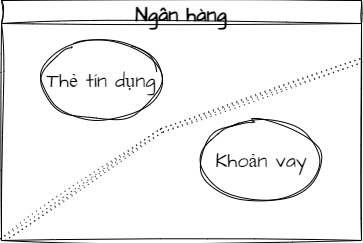
\includegraphics[scale = 0.5]{pictures/mo_hinh_rieng_biet_separate_ways/main.drawio.png}

\caption{Ví dụ mô hình riêng biệt (Separate Ways)}

\end{figure}

\end{example}


\subsubsection{Ngôn ngữ được xuất bản (Published Language)}
 
Khi   ngôn ngữ chung ở     dịch vụ máy chủ mở  được các nhóm phát triển trong     bối cảnh giới hạn  hạ lưu chấp nhận.   Ngôn ngữ chung này được gọi là  ngôn ngữ được xuất bản (Published Language). Ngôn ngữ  được xuất bản có lợi ích là tính thống nhất trong hệ thống tuy nhiên cần phân tích kĩ  vì nó có thể tạo ra  sự nhầm lẫn trong     bối cảnh giới hạn hạ lưu   nào đó.
Trong bản đồ    bối cảnh,     ngôn ngữ được xuất bản kết hợp dịch vụ máy chủ mở    được ký hiệu là     OHS|PL.
 
 
     
%%%%%%%%%%%%%%%%%%%%%%%%%%%%%%%%%%
%%%%%%%%%%%%%%%%%%%%%%%%%%%%%%%%%%
%%%%%%%%%%%%%%%%%%%%%%%%%%%%%%%%%%
%%%%%%%%%%%%%%%%%%%%%%%%%%%%%%%%%%
%%%%%%%%%%%%%%%%%%%%%%%%%%%%%%%%%%
%%%%%%%%%%%%%%%%%%%%%%%%%%%%%%%%%%
%%%%%%%%%%%%%%%%%%%%%%%%%%%%%%%%%%
%%%%%%%%%%%%%%%%%%%%%%%%%%%%%%%%%%

% \section{Áp dụng về các mối quan hệ bối cảnh giới hạn}
%! Hướng dẫn 6/6

%%%%%%%%%%%%%%%%%%%%%%%%%%%%%%%%%%

%%%%%%%%%%%%%%%%%%%%%%%%%%%%%%%%%%

%%%%%%%%%%%%%%%%%%%%%%%%%%%%%%%%%%

%%%%%%%%%%%%%%%%%%%%%%%%%%%%%%%%%%

%%%%%%%%%%%%%%%%%%%%%%%%%%%%%%%%%%

%%%%%%%%%%%%%%%%%%%%%%%%%%%%%%%%%%

%%%%%%%%%%%%%%%%%%%%%%%%%%%%%%%%%%

%%%%%%%%%%%%%%%%%%%%%%%%%%%%%%%%%%

% \chapter{Các mẫu kỹ thuật}

% Các mẫu     kỹ thuật được sử dụng để lập mô hình và hiện thực hóa  các thành phần riêng lẻ của hệ thống microservices.  Các mẫu     kỹ thuật  tập trung    mô hình hóa miền và triển khai logic nghiệp vụ trong lập trình.




 

Các yếu tố  các mẫu     kỹ thuật  bao gồm:





\begin{itemize}
\item Muc1  
\item Muc1  
\item Muc1  
\item Muc1  
\item Muc1  
\item Muc1  
\item Muc1  
\item Muc1  
\item Muc1  
\item Muc2  
\end{itemize}






  

%!<! - - $ Vẽ lại sau: - - >

%!<! - - $ Vẽ lại sau: - - >

%!<! - - $ Vẽ lại sau: - - >

%!<! - - $ Vẽ lại sau: - - >

%!<! - - $ Vẽ lại sau: - - >

%!<! - - $ Vẽ lại sau: - - >

%!<! - - $ Vẽ lại sau: - - >

%!<! - - $ Vẽ lại sau: - - >

%!<! - - $ Vẽ lại sau: - - >

%!<! - - $ Vẽ lại sau: - - >

%!<! - - $ Vẽ lại sau: - - >

%!<! - - $ Vẽ lại sau: - - >

%!<! - - $ Vẽ lại sau: - - >

% \section{Các đối tượng miền (Domain Object)}

% Đối tượng miền (Domain Object)    được sử dụng để mô hình hóa    mô hình miền.  Đối tượng miền    được sử dụng để   triển khai   các quy tắc, các ràng buộc và các mối quan hệ   của nghiệp vụ.
Đối tượng miền   bao gồm:





\begin{itemize}
\item Đối tượng thực thể (Entities Objects)  
\item Đối tượng giá trị (Value Objects) 
\item  Miền dịch vụ (Service Domain) 

\end{itemize}

 
 
 

 

% \subsection{Đối tượng thực thể (Entities Objects)}

% 
% Đối tượng miền có thể là một thực thể, là đối tượng miền có nhận dạng duy nhất hoặc đối tượng giá trị, là đối tượng đại diện cho một đặc điểm của miền mà không có nhận dạng riêng.


% Đối tượng thực thể có bản sắc riêng nhưng không thể

% tồn tại nếu không có tập hợp gốc, nghĩa là chúng

% được tạo khi tập hợp gốc được tạo và bị hủy khi tập

% hợp gốc bị phá hủy.

% Đối tượng thực thể = Mã định danh phụ của Bối cảnh giới hạn của chúng ta

%! % Entity Object -

****

% ****

Trong các đối tượng của một phần mềm, có một nhóm các đối tượng có định danh riêng.

Định danh này được giữ nguyên xuyên suốt trạng thái hoạt động của phần mềm. Hệ thống phân biệt hai đối tượng với hai định danh khác nhau, hay hai đối tượng chung định danh có thể coi là một.

Các thực thể là những đối tượng rất quan trọng của mô hình miền. Việc xác định xem một đối tượng có phải là thực thể hay không rất quan trọng.

Trong trường hợp CSDL quan hệ, một bảng biểu thị một tập hợp các thực thể. Các quy tắc trong bảng biểu thị các thực thể được xác định duy nhất bằng cột khóa chính.

Hành vi này triển khai logic nghiệp vụ có thể thay đổi trạng thái của thực thể. Các thực thể được lưu trữ lâu dài.

% %! Entity : https:// thiết kế hướng miền - practitioners.com/entity

% %! Entity : https:// thiết kế hướng miền - practitioners.com/entity

% %! Entity : https:// thiết kế hướng miền - practitioners.com/entity

% %! Entity : https:// thiết kế hướng miền - practitioners.com/entity


thực thể

Trong Thiết kế hướng miền (thiết kế hướng miền), thực thể là khái niệm cốt lõi đại diện cho một đối tượng miền có nhận dạng duy nhất. Thực thể là một đối tượng được phân biệt với các đối tượng khác dựa trên nhận dạng duy nhất của nó, thay vì thuộc tính hoặc giá trị của nó.

Các thực thể thường là các đối tượng quan trọng nhất trong mô hình miền và chúng thường có logic và hành vi nghiệp vụ phức tạp được liên kết với chúng. Họ cũng có thể có mối quan hệ với các thực thể, đối tượng giá trị hoặc dịch vụ miền khác.

Một thực thể có các đặc điểm sau:

Danh tính: Một thực thể có một danh tính duy nhất để phân biệt nó với các thực thể khác trong mô hình miền. Danh tính thường được biểu thị bằng ID hoặc khóa, chẳng hạn như ID khách hàng hoặc SKU sản phẩm.

Khả năng thay đổi: Các thuộc tính của thực thể có thể thay đổi theo thời gian trong khi vẫn duy trì được danh tính của nó. Ví dụ: tên hoặc địa chỉ của khách hàng có thể thay đổi nhưng ID khách hàng vẫn giữ nguyên.

Hành vi: Một thực thể có hành vi liên quan đến nó, thường là các quy tắc và logic nghiệp vụ phức tạp. Hành vi này thường được gói gọn trong chính thực thể đó.

Mối quan hệ: Một thực thể có thể có mối quan hệ với các thực thể, đối tượng giá trị hoặc dịch vụ miền khác. Ví dụ: khách hàng có thể có lịch sử đặt hàng hoặc giỏ hàng.

Các thực thể là một phần thiết yếu của mô hình miền và phải được thiết kế để thể hiện chính xác miền và các quy tắc kinh doanh của nó. Bằng cách lập mô hình chính xác các thực thể, nhà phát triển có thể tạo ra giải pháp phần mềm linh hoạt và dễ bảo trì hơn, đáp ứng nhu cầu của miền.

Một ví dụ

Hãy xem xét một nền tảng thương mại điện tử nơi khách hàng có thể đặt hàng sản phẩm. Trong mô hình miền này, Đơn hàng là một thực thể. Mỗi đơn hàng có một danh tính duy nhất và bất biến, chẳng hạn như số đơn hàng, giúp phân biệt nó với các đơn hàng khác trong hệ thống.

Thực thể Đơn hàng có thể có một số thuộc tính, chẳng hạn như thông tin khách hàng, chi tiết thanh toán và thông tin giao hàng. Nó cũng có thể có mối quan hệ với các thực thể khác, chẳng hạn như thực thể Sản phẩm và Khách hàng.

Hành vi của thực thể Đơn hàng bao gồm tạo và cập nhật đơn hàng, quản lý xử lý thanh toán và theo dõi trạng thái đơn hàng.

Dưới đây là ví dụ về giao diện của thực thể Đơn hàng trong mã:

public class Order {

private OrderId orderId;

private Customer customer;

private List<Product> products;

private Date orderDate;

private PaymentDetails paymentDetails;

private ShippingDetails shippingDetails;

public Order(OrderId orderId, Customer customer) {

this.orderId = orderId;

this.customer = customer;

this.products = Lists.newArrayList();

this.orderDate = LocalDate.now();

}

public void addProduct(Product product) {

products.add(product);

}

public void removeProduct(Product product) {

products.remove(product);

}

public void processPayment() {

// Process payment logic here...

}

public void shipOrder() {

// Shipping logic here...

}

// Other behavior methods here...

}

Trong ví dụ này, thực thể Đơn hàng có một ID duy nhất (orderId) xác định nó trong hệ thống, cùng với các thuộc tính khác như customer, < /span>, gói gọn logic kinh doanh được liên kết với thực thể đơn hàng., và,, . Thực thể cũng có các phương thức hành vi, chẳng hạn như và, products, orderDatepaymentDetailsshippingDetailsaddProductremoveProductprocessPaymentshipOrder

% %! Entity : https:// thiết kế hướng miền - practitioners.com/entity

% %! Entity : https:// thiết kế hướng miền - practitioners.com/entity

% %! Entity : https:// thiết kế hướng miền - practitioners.com/entity


% %! Entity Identity : https:// thiết kế hướng miền - practitioners.com/entity - identity

% %! Entity Identity : https:// thiết kế hướng miền - practitioners.com/entity - identity

% %! Entity Identity : https:// thiết kế hướng miền - practitioners.com/entity - identity

% %! Entity Identity : https:// thiết kế hướng miền - practitioners.com/entity - identity

Trang chủTrang chủBảng chú giảiNhận dạng thực thể

Nhận dạng thực thể

Danh tính của một thực thể phải là duy nhất và bất biến, nghĩa là nó không được thay đổi trong suốt vòng đời của thực thể đó. Việc thay đổi danh tính của một thực thể có thể gây ra hậu quả nghiêm trọng, chẳng hạn như gây ra sự không nhất quán về dữ liệu hoặc phá vỡ mối quan hệ với các thực thể hoặc đối tượng giá trị khác. Ví dụ: nếu ID của khách hàng bị thay đổi, điều đó có thể dẫn đến nhầm lẫn khi theo dõi lịch sử mua hàng của họ hoặc các tương tác khác với hệ thống.

Điều quan trọng cần lưu ý là các thuộc tính của thực thể, chẳng hạn như tên hoặc địa chỉ, có thể thay đổi mà không ảnh hưởng đến danh tính của thực thể đó. Những thay đổi này phải được quản lý thông qua việc đóng gói thích hợp hành vi và logic kinh doanh của thực thể.

Tóm lại, danh tính của một thực thể phải là duy nhất và bất biến, đồng thời những thay đổi đối với các thuộc tính của thực thể sẽ không ảnh hưởng đến danh tính của thực thể đó. Bằng cách tuân thủ nguyên tắc này, các nhà phát triển có thể tạo ra một mô hình miền nhất quán và dễ bảo trì hơn, thể hiện chính xác miền kinh doanh.

Làm thế nào để chọn một danh tính thực thể tốt

Chọn danh tính phù hợp cho một thực thể là một phần quan trọng trong việc thiết kế mô hình miền trong Thiết kế hướng miền (thiết kế hướng miền). Dưới đây là một số phương pháp hay để chọn danh tính của một thực thể:

Chọn một danh tính duy nhất: Danh tính của một thực thể phải là duy nhất trong mô hình miền và nó không được thay đổi trong suốt vòng đời của thực thể. Danh tính của một thực thể phải được xác định theo yêu cầu kinh doanh, chẳng hạn như mã định danh duy nhất như số sê - ri, ID khách hàng hoặc số an sinh xã hội.

Chọn danh tính ổn định: Danh tính của thực thể phải ổn định, nghĩa là danh tính không được thay đổi theo thời gian. Danh tính ổn định cho phép tính nhất quán và độ chính xác trong mô hình miền và nó có thể ngăn ngừa lỗi trong hệ thống. Ví dụ: nếu ID của khách hàng thay đổi, việc theo dõi lịch sử mua hàng của họ hoặc các tương tác khác với hệ thống có thể gây nhầm lẫn.

Chọn danh tính dễ nhận dạng: Danh tính của thực thể phải dễ nhận dạng, tốt nhất là bởi người đọc. Ví dụ: việc sử dụng UUID hoặc GUID có thể không dễ nhận biết như tên hoặc số ID của khách hàng.

Chọn một danh tính có thể được sử dụng nhất quán trong toàn bộ mô hình miền: Danh tính của một thực thể phải nhất quán trong toàn bộ mô hình miền và nó phải được sử dụng nhất quán trong mọi ngữ cảnh mà thực thể đó được tham chiếu.

Xem xét khả năng mở rộng và hiệu suất: Việc chọn một danh tính có thể mở rộng quy mô và hoạt động tốt cũng rất quan trọng, đặc biệt đối với các hệ thống có khối lượng dữ liệu lớn hoặc thông lượng cao.

Bằng cách làm theo những thực tiễn này, nhà phát triển có thể chọn danh tính phù hợp cho các thực thể thể hiện chính xác mô hình miền và cung cấp giải pháp phần mềm linh hoạt và có thể bảo trì.

% %! Entity Identity : https:// thiết kế hướng miền - practitioners.com/entity - identity

% %! Entity Identity : https:// thiết kế hướng miền - practitioners.com/entity - identity

% %! Entity Identity : https:// thiết kế hướng miền - practitioners.com/entity - identity

% %! Entity Identity : https:// thiết kế hướng miền - practitioners.com/entity - identity



% \subsection{Đối tượng giá trị (Value Objects)}

% % Một đối tượng được dùng để mô tả các khía cạnh cố định của một miền và không có định danh.

% Đối tượng giá trị không có danh tính duy nhất.

% Đối tượng giá trị được tạo trong bộ nhớ tiến trình và sau đó bị hủy sau khi nó đã phục vụ mục đích của nó.

% Một điểm khác biệt quan trọng giữa các thực thể và đối tượng giá trị là đối tượng giá trị không tồn tại lâu dài trong CSDL.

% %! VD

% %! chúng ta sẽ đặt logic xác thực cho địa chỉ email ở đâu?

% %! xác nhận kỹ thuật không liên quan đến bất kỳ khái niệm kinh doanh nào.

% %! tạo một đối tượng giá trị để xác thực địa chỉ email.

% %! Kết quả là, thực thể khách hàng sẽ sạch hơn và đơn giản hơn nhiều trong việc thực hiện.

% %! % Value Object -

% %! Value Object : https:// thiết kế hướng miền - practitioners.com/home/glossary/value - object

% %! Value Object : https:// thiết kế hướng miền - practitioners.com/home/glossary/value - object

% %! Value Object : https:// thiết kế hướng miền - practitioners.com/home/glossary/value - object

% %! [[Value Object]] An object that describes some characteristic or attribute but carries no concept of identity.

Trang chủTrang chủBảng chú giảiĐối tượng giá trị

Đối tượng giá trị

Trong Thiết kế hướng miền (thiết kế hướng miền), đối tượng giá trị là một đối tượng đại diện cho một khái niệm hoặc ý tưởng trong mô hình miền không có danh tính duy nhất hoặc tuổi thọ vượt quá tuổi thọ của thực thể chứa đối tượng.

Một đối tượng giá trị được xác định bởi các thuộc tính của nó và nó không thể thay đổi, nghĩa là trạng thái của nó không thể thay đổi sau khi được tạo. Các đối tượng giá trị thường được sử dụng để biểu thị số lượng, phép đo, ngày tháng, tiền tệ hoặc các khái niệm khác có thể được biểu thị dưới dạng kết hợp các thuộc tính.

Vì các đối tượng giá trị không có danh tính duy nhất nên chúng có thể được sao chép và chia sẻ tự do mà không ảnh hưởng đến tính nhất quán của mô hình miền. Các đối tượng giá trị cũng được so sánh dựa trên thuộc tính của chúng chứ không phải danh tính của chúng, điều này cho phép so sánh linh hoạt và trực quan hơn.

Trong triển khai phần mềm, các đối tượng giá trị thường được tạo dưới dạng các lớp bất biến, không có danh tính riêng và chúng thường được triển khai như một phần của thực thể hoặc tập hợp chứa. Bằng cách sử dụng các đối tượng giá trị trong mô hình miền, nhà phát triển có thể tạo mã có tính biểu cảm hơn, dễ bảo trì và mở rộng hơn để phản ánh tốt hơn miền kinh doanh.

Một ví dụ

Giả sử chúng ta đang xây dựng một trang web thương mại điện tử và chúng ta có yêu cầu thể hiện giá trong mô hình miền. Giá là một ứng cử viên phù hợp cho đối tượng giá trị vì nó có thể được biểu diễn dưới dạng kết hợp các thuộc tính (ví dụ: tiền tệ và số lượng) và không có đặc điểm nhận dạng duy nhất của riêng nó.

Đây là một ví dụ cực kỳ đơn giản về đối tượng Giá trị giá trong Java:

1

2

3

4

5

6

7

số 8

9

10

11

12

13

14

15

16

17

18

19

class Price {

private final Currency currency;

private final BigDecimal amount;

public Price(Currency currency, BigDecimal amount) {

this.currency = currency;

this.amount = amount;

}

public Currency getCurrency() {

return currency;

}

public BigDecimal getAmount() {

return amount;

}

// Other methods and business logic specific to the Price concept

}

Trong ví dụ này, đối tượng giá trị Price có hai thuộc tính: currency và amount. Thuộc tính currency đại diện cho đơn vị tiền tệ của giá (ví dụ: USD, EUR, v.v.), trong khi thuộc tính amount đại diện cho giá trị bằng số của giá. Đối tượng Price là bất biến và trạng thái của nó không thể thay đổi sau khi được tạo. Đối tượng Price cũng xác định các phương thức để truy xuất các thuộc tính của nó (ví dụ: getCurrency() và getAmount()), cũng như các phương thức khác dành riêng cho < khái niệm /span>). hoặc Price (ví dụ: phương thức add()subtract()

Bằng cách sử dụng đối tượng giá trị Price, chúng tôi có thể đảm bảo rằng giá được thể hiện nhất quán trong toàn bộ mô hình miền và chúng tôi có thể thực hiện các so sánh và tính toán linh hoạt và trực quan hơn về giá.

Đối tượng giá trị so với thực thể

Đối tượng giá trị trong một giải pháp có thể trở thành một thực thể trong giải pháp khác. Sự khác biệt giữa các đối tượng giá trị và các thực thể phụ thuộc vào ngữ cảnh và dựa trên nhu cầu của mô hình miền.

Trong một ngữ cảnh, một đối tượng có thể được coi là một đối tượng giá trị vì nó được xác định bởi các thuộc tính của nó và không có một danh tính duy nhất. Tuy nhiên, trong một bối cảnh khác hoặc một giải pháp khác, cùng một đối tượng có thể được coi là một thực thể vì nó có một danh tính duy nhất và có thể được lưu giữ trong CSDL hoặc có tuổi thọ vượt quá đối tượng chứa.

Ví dụ: hãy xem xét một đối tượng Person trong miền nhân sự. Trong một ngữ cảnh, đối tượng Person có thể được coi là một đối tượng giá trị vì nó được xác định bởi các thuộc tính của nó, chẳng hạn như tên, ngày sinh và số an sinh xã hội. Tuy nhiên, trong một ngữ cảnh khác hoặc một giải pháp khác, đối tượng Person có thể được coi là một thực thể vì nó có một danh tính duy nhất và có thể được duy trì trong CSDL hoặc được sử dụng trên các ngữ cảnh giới hạn khác nhau.

Cuối cùng, việc lựa chọn mô hình hóa một đối tượng là đối tượng giá trị hay thực thể phụ thuộc vào nhu cầu của mô hình miền và các yêu cầu cụ thể của giải pháp phần mềm đang được phát triển. Điều quan trọng là chọn các khái niệm mô hình phù hợp để thể hiện chính xác miền và cung cấp giải pháp phần mềm linh hoạt và có thể bảo trì.

% %! Value Object : https:// thiết kế hướng miền - practitioners.com/home/glossary/value - object

% %! Value Object : https:// thiết kế hướng miền - practitioners.com/home/glossary/value - object

% %! Value Object : https:// thiết kế hướng miền - practitioners.com/home/glossary/value - object



% \subsection{Miền dịch vụ (Service)}

% % %! Service : https:// thiết kế hướng miền - practitioners.com/ dịch vụ

% %! Service : https:// thiết kế hướng miền - practitioners.com/ dịch vụ

% %! Service : https:// thiết kế hướng miền - practitioners.com/ dịch vụ

% %! Service : https:// thiết kế hướng miền - practitioners.com/ dịch vụ

% %! Service : https:// thiết kế hướng miền - practitioners.com/ dịch vụ

% %! [[Service]] An operation offered as an interface that stands alone in the model, with no encapsulated state.

Chuyển đến nội dung

Đối với người hành nghề bởi người hành nghề

Tìm kiếm

Thiết kế hướng miền: Hướng dẫn dành cho người thực hành

Câu hỏi thường gặp

Bảng chú giải

Về chúng tôi

Cuốn sách của chúng tôi!

Trang chủTrang chủBảng chú giảiDịch vụ

Dịch vụ

Trong thiết kế hướng miền, dịch vụ là một phần của lớp miền triển khai logic miền hoặc trường hợp sử dụng không phù hợp một cách tự nhiên với một thực thể hoặc đối tượng giá trị cụ thể. Nó thường điều phối các tương tác giữa nhiều thực thể hoặc tập hợp. Một dịch vụ đại diện cho một hoạt động gắn kết và không trạng thái có đầu vào và đầu ra. Nó không có trạng thái bền vững và không cần phải khởi tạo. Các dịch vụ thường có tên phản ánh mục đích miền của chúng, chẳng hạn như `OrderProcessingService` hoặc `PaymentService`.

Có một số trường hợp nhất định mà việc sử dụng dịch vụ có thể không phù hợp.

Thứ nhất, nếu logic nghiệp vụ có thể được liên kết với một thực thể hoặc đối tượng giá trị, có thể tốt hơn nếu gói gọn logic trong thực thể hoặc đối tượng giá trị đó. Điều này có thể giúp cải thiện tính gắn kết của mã và làm cho mã dễ hiểu hơn.

Thứ hai, nếu logic nghiệp vụ liên quan đến nhiều thực thể hoặc tập hợp được liên kết chặt chẽ với nhau thì tốt hơn là chúng ta nên đánh giá lại thiết kế của bản thân các uẩn. Trong những trường hợp như vậy, có thể phù hợp hơn nếu phân chia các tập hợp hoặc xác định lại ranh giới của chúng để giảm sự ghép nối và cải thiện khả năng bảo trì.

Cuối cùng, nếu logic nghiệp vụ liên quan đến các hệ thống hoặc cơ sở hạ tầng bên ngoài thì tốt hơn nên sử dụng lớp chống đổ vỡ hoặc mẫu bộ chuyển đổi để tách biệt mô hình miền khỏi các phụ thuộc bên ngoài. Điều này có thể giúp giảm khả năng ghép nối và cải thiện tính linh hoạt của hệ thống.

Ví dụ

Dưới đây là ví dụ về một dịch vụ trong Java có liên quan đến nhiều hơn một tổng hợp:

1

2

3

4

5

6

7

số 8

9

10

11

12

13

14

15

public class OrderService {

private final OrderRepository orderRepository;

private final ProductRepository productRepository;

public void createOrder(Order order) {

for (OrderItem item: order.getItems()) {

Product product = productRepository.findById(item.getProductId());

product.reduceStockBy(item.getQuantity());

productRepository.save(product);

}

orderRepository.save(order);

}

// Other methods...

}

Trong ví dụ này, OrderService chịu trách nhiệm tạo đơn đặt hàng và nó tương tác với hai tập hợp: Order và Product. Tổng hợp Order đại diện cho đơn đặt hàng do khách hàng đặt, trong khi tổng hợp Product đại diện cho một sản phẩm có thể được đặt hàng.

Phương thức createOrder cập nhật kho của từng sản phẩm trong đơn hàng bằng cách gọi phương thức save trên ProductRepository, và sau đó tự lưu đơn hàng bằng cách gọi phương thức save trên OrderRepository.

Thể loại

Phân tích

điều cơ bản

thiết kế hướng miền

thiết kế

câu hỏi thường gặp

Khả năng lãnh đạo

hoa văn

Blog tại WordPress.com.

% %! Service : https:// thiết kế hướng miền - practitioners.com/ dịch vụ

% %! Service : https:// thiết kế hướng miền - practitioners.com/ dịch vụ

% %! Service : https:// thiết kế hướng miền - practitioners.com/ dịch vụ

% %! Service : https:// thiết kế hướng miền - practitioners.com/ dịch vụ

% %! Service : https:// thiết kế hướng miền - practitioners.com/ dịch vụ

% %! Service : https:// thiết kế hướng miền - practitioners.com/ dịch vụ



% %! Hướng dẫn 7/4

% %! Hướng dẫn 7/5

% \subsubsection{xxxxxxx}

% 

% Vẽ lại bản đồ tiếng Việt
% Vẽ lại bản đồ tiếng Việt
% Vẽ lại bản đồ tiếng Việt
% Vẽ lại bản đồ tiếng Việt
% Vẽ lại bản đồ tiếng Việt
% Vẽ lại bản đồ tiếng Việt
% Vẽ lại bản đồ tiếng Việt
% Vẽ lại bản đồ tiếng Việt
% Từ bản đồ lấy vi dụ cho các mô hình
% Từ bản đồ lấy vi dụ cho các mô hình
% Từ bản đồ lấy vi dụ cho các mô hình
% Từ bản đồ lấy vi dụ cho các mô hình
% Từ bản đồ lấy vi dụ cho các mô hình
% Từ bản đồ lấy vi dụ cho các mô hình
% Từ bản đồ lấy vi dụ cho các mô hình
% Từ bản đồ lấy vi dụ cho các mô hình
% Từ bản đồ lấy vi dụ cho các mô hình
% Từ bản đồ lấy vi dụ cho các mô hình
\begin{example} Trong miền vấn đề ngân hàng,     thẻ tín dụng và khoản vay mua nhà không có mối quan hệ. 
    
    \begin{figure}[H]
        
        \centering
        
        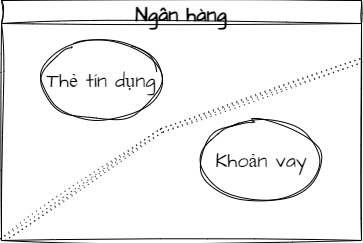
\includegraphics[scale = 0.5]{pictures/mo_hinh_rieng_biet_separate_ways/main.drawio.png}
        
        \caption{Ví dụ  mô hình riêng biệt (Separate Ways)  }
        
    \end{figure}
\end{example} 

% %! $VD: hình giao như 2 tập hợp - - >

%%%%%%%%%%%%%%%%%%%%%%%%%%%%%%%%%%

\end{document} % Kết thúc

% kết luận, tài liệu tham khảo

%%%%%%%%%%%%%%%%%%%%%%%%%%%%%%%%%%

% % %! Aggregates/ /

% % Tổng hợp là đối tượng kinh doanh trung tâm trong Bối cảnh giới hạn của chúng ta và xác định phạm vi nhất quán trong bối cảnh giới hạn đó.

% % Tổng hợp = Mã định danh chính của Bối cảnh giới hạn của chúng ta

% \subsubsection{xxxxxxx}

% % 

% Vẽ lại bản đồ tiếng Việt
% Vẽ lại bản đồ tiếng Việt
% Vẽ lại bản đồ tiếng Việt
% Vẽ lại bản đồ tiếng Việt
% Vẽ lại bản đồ tiếng Việt
% Vẽ lại bản đồ tiếng Việt
% Vẽ lại bản đồ tiếng Việt
% Vẽ lại bản đồ tiếng Việt
% Từ bản đồ lấy vi dụ cho các mô hình
% Từ bản đồ lấy vi dụ cho các mô hình
% Từ bản đồ lấy vi dụ cho các mô hình
% Từ bản đồ lấy vi dụ cho các mô hình
% Từ bản đồ lấy vi dụ cho các mô hình
% Từ bản đồ lấy vi dụ cho các mô hình
% Từ bản đồ lấy vi dụ cho các mô hình
% Từ bản đồ lấy vi dụ cho các mô hình
% Từ bản đồ lấy vi dụ cho các mô hình
% Từ bản đồ lấy vi dụ cho các mô hình
\begin{example} Trong miền vấn đề ngân hàng,     thẻ tín dụng và khoản vay mua nhà không có mối quan hệ. 
    
    \begin{figure}[H]
        
        \centering
        
        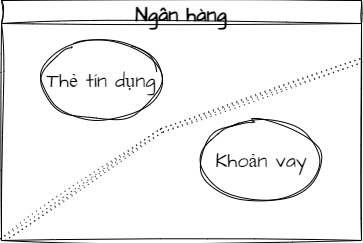
\includegraphics[scale = 0.5]{pictures/mo_hinh_rieng_biet_separate_ways/main.drawio.png}
        
        \caption{Ví dụ  mô hình riêng biệt (Separate Ways)  }
        
    \end{figure}
\end{example} 

% %! $VD: hình giao như 2 tập hợp - - >

% \end{document} % kết thúc

% Yêu cầu nghiệp vụ của từng sub

% %

% Sơ đồ if else Đ S

% %

% sub trước model

% %

%%%%%%%%%%%%%%%%%%%%%%%%%%%%%%%%%%%%%

\end{document}

\section{xxxxxxx}

\subsection{xxxxxxx}

\subsubsection{xxxxxxx}



% Vẽ lại bản đồ tiếng Việt
% Vẽ lại bản đồ tiếng Việt
% Vẽ lại bản đồ tiếng Việt
% Vẽ lại bản đồ tiếng Việt
% Vẽ lại bản đồ tiếng Việt
% Vẽ lại bản đồ tiếng Việt
% Vẽ lại bản đồ tiếng Việt
% Vẽ lại bản đồ tiếng Việt
% Từ bản đồ lấy vi dụ cho các mô hình
% Từ bản đồ lấy vi dụ cho các mô hình
% Từ bản đồ lấy vi dụ cho các mô hình
% Từ bản đồ lấy vi dụ cho các mô hình
% Từ bản đồ lấy vi dụ cho các mô hình
% Từ bản đồ lấy vi dụ cho các mô hình
% Từ bản đồ lấy vi dụ cho các mô hình
% Từ bản đồ lấy vi dụ cho các mô hình
% Từ bản đồ lấy vi dụ cho các mô hình
% Từ bản đồ lấy vi dụ cho các mô hình
\begin{example} Trong miền vấn đề ngân hàng,     thẻ tín dụng và khoản vay mua nhà không có mối quan hệ. 
    
    \begin{figure}[H]
        
        \centering
        
        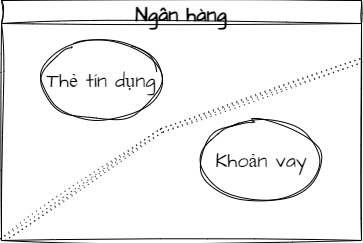
\includegraphics[scale = 0.5]{pictures/mo_hinh_rieng_biet_separate_ways/main.drawio.png}
        
        \caption{Ví dụ  mô hình riêng biệt (Separate Ways)  }
        
    \end{figure}
\end{example} 

% %! $VD: hình giao như 2 tập hợp - - >

% phải có CQRS (Phân chia trách nhiệm truy vấn lệnh)

CQRS là một mẫu kiến trúc riêng biệt có thể được sử dụng kết hợp với thiết kế hướng miền để đạt được những lợi ích nhất định, chẳng hạn như cải thiện hiệu suất và khả năng mở rộng. Tuy nhiên, nó không phải là một yêu cầu để triển khai thiết kế hướng miền.

% phải có event

Ngôn ngữ chung (Ubiquitous Language)

%%%%%%%%%%%%%%%%%%%%%%%%%%%%%%%%%%%%%

\end{document} % kết thúc

Cách tiếp cận này nhấn mạnh tính mô - đun, tính linh hoạt và khả năng phục hồi, cho phép các nhóm làm việc đồng thời trên các phần khác nhau của hệ thống và cho phép phát hành nhanh hơn và thường xuyên hơn. Các vi dịch vụ thường dựa vào các giao thức truyền thông nhẹ, chẳng hạn như REST và thường được triển khai bằng các công nghệ chứa trong bộ chứa như Docker và Kubernetes.

\subsubsection{DevOps Ứng dụng, áp dụng, liên quan,....}

\subsubsection{CI/CD}

\subsubsection{Docker}

\subsubsection{Kubernetes}

dícovery

api gateway

%@ Tất cả phải dùng ulli